%% ============================================================
%%  An Autonomous Decision Framework for Resource-Constrained
%%  Exoplanet Characterization Campaigns
%% ============================================================
\documentclass[11pt,a4paper]{article}

%% ---- Packages -----------------------------------------------
\usepackage[margin=2.2cm]{geometry}
\usepackage{amsmath,amssymb,amsthm}
\usepackage{graphicx}
\usepackage{booktabs}
\usepackage{array}
\usepackage{longtable}
\usepackage{multirow}
\usepackage{xcolor}
\usepackage{hyperref}
\usepackage{caption}
\usepackage{subcaption}
\usepackage{float}
\usepackage{listings}
\usepackage{setspace}
\usepackage{fancyhdr}
\usepackage{titlesec}
% \usepackage{microtype} 

%% ---- Color palette (Academic Preprint Style) ----------------
\definecolor{deepblue}{RGB}{15,23,42}
\definecolor{tealaccent}{RGB}{13,148,136}
\definecolor{goldcolor}{RGB}{217,119,6}
\definecolor{pinkcolor}{RGB}{156,163,175}
\definecolor{lightblue}{RGB}{3,105,161}
\definecolor{mutedgray}{RGB}{71,85,105}
\definecolor{codebg}{RGB}{248,250,252}

%% ---- Hyperref setup -----------------------------------------
\hypersetup{
    colorlinks=true,
    linkcolor=lightblue,
    citecolor=tealaccent,
    urlcolor=lightblue,
    pdftitle={A Simulation Framework for Adaptive Multi-Objective Scheduling of Exoplanet Characterization Campaigns},
    pdfauthor={Rushikesh},
}

%% ---- Header/footer ------------------------------------------
\pagestyle{fancy}
\fancyhf{}
\rhead{\small Exoplanet Prioritization \& Active Scheduling}
\lhead{\small Rushikesh}
\cfoot{\thepage}
\renewcommand{\headrulewidth}{0.4pt}

%% ---- Section formatting ------------------------------------
\titleformat{\section}{\large\bfseries\color{deepblue}}{\thesection}{1em}{}[\titlerule]
\titleformat{\subsection}{\normalsize\bfseries\color{lightblue}}{\thesubsection}{1em}{}
\titleformat{\subsubsection}{\normalsize\itshape\color{tealaccent}}{\thesubsubsection}{1em}{}

%% ---- Code listing style ------------------------------------
\lstset{
    backgroundcolor=\color{codebg},
    basicstyle=\ttfamily\footnotesize\color{deepblue},
    keywordstyle=\color{tealaccent}\bfseries,
    commentstyle=\color{mutedgray}\itshape,
    stringstyle=\color{goldcolor},
    breaklines=true,
    frame=single,
    rulecolor=\color{pinkcolor},
    numbers=left,
    numberstyle=\tiny\color{mutedgray},
    language=Python,
    showstringspaces=false,
}

%% ---- Custom boxes -------------------------------------------
\newsavebox{\noveltySaveBox}
\newenvironment{noveltybox}
  {\begin{lrbox}{\noveltySaveBox}\begin{minipage}{\dimexpr\textwidth-2\fboxsep-2\fboxrule\relax}}
  {\end{minipage}\end{lrbox}\begin{center}\fcolorbox{tealaccent}{tealaccent!5}{\usebox{\noveltySaveBox}}\end{center}}

\newsavebox{\formulaSaveBox}
\newenvironment{formulabox}
  {\begin{lrbox}{\formulaSaveBox}\begin{minipage}{\dimexpr\textwidth-2\fboxsep-2\fboxrule\relax}}
  {\end{minipage}\xdef\useFormulaSaveBox{\usebox{\formulaSaveBox}}\end{lrbox}\begin{center}\fcolorbox{goldcolor}{goldcolor!5}{\usebox{\formulaSaveBox}}\end{center}}

%% ============================================================
\begin{document}

%% ---- Title & Metadata ---------------------------------------
\title{\textbf{A Simulation Framework for Adaptive Multi-Objective Scheduling of Exoplanet Characterization Campaigns}}

\author{
    \textbf{Rushikesh} \\
    \small Data Source: NASA Exoplanet Archive (TAP API) \\
    \small GitHub Repository: \href{https://github.com/rushikesh-D69/water}{rushikesh-D69/water}
}

\date{\today}

\maketitle

\onehalfspacing

\begin{abstract}
Spectroscopic characterization of exoplanet atmospheres is expensive in telescope time. Static target lists do not react to time-varying visibility or weather, and single-objective greedy policies concentrate on easy-to-observe mini-Neptunes. This paper describes a \emph{simulation} framework and scheduling policy for that setting; it does not evaluate JWST or Habitable Worlds Observatory operations.

Stage~1 constructs a continuous priority score from habitable-zone flux limits, a rocky-composition proxy, and an Earth Similarity Index, then trains tree ensembles to recover that score from NASA Exoplanet Archive catalog columns. Because the label is a deterministic function of those columns, near-perfect ranking is expected and is not evidence of independent astrophysical inference. Ensemble variance is used only as a cheap exploration signal for Stage~2.

Stage~2 treats campaign execution as constrained sequential selection under simulated visibility and an AR(1) weather process. An exponential weight-decay schedule mixes exploration, priority, and detectability. Across 20 simulated campaigns, the adaptive policy outperforms static and single-objective greedy baselines on a composite of gain, diversity, efficiency, and priority coverage (mean $\pm$ standard deviation). A perfect-knowledge Oracle that optimizes the same utility is an implementation check, not a generalization test.

Code, pinned dependencies, random seeds, and the NASA TAP snapshot date (2026-05-26) are recorded in the repository.
\end{abstract}

\newpage

%% ============================================================
\section{Introduction}
\label{sec:intro}

The discovery of exoplanets has become a statistical astronomical discipline. Radial-velocity surveys and transit missions, notably Kepler and the Transiting Exoplanet Survey Satellite (TESS) \cite{barclay2018}, have confirmed thousands of planets. Catalogs now contain a wide range of architectures, masses, and host stars.

The scarce resource is spectroscopic characterization, not detection. Transmission and emission spectroscopy require much higher signal-to-noise than a transit detection, often tens or hundreds of hours on a single target to constrain species such as $\mathrm{H_2O}$, $\mathrm{CO_2}$, $\mathrm{CH_4}$, or $\mathrm{O_3}$.

Flagship facilities, including the James Webb Space Telescope (JWST) and concepts such as the Habitable Worlds Observatory (HWO), allocate only a fraction of their time to exoplanet spectroscopy. Target choice and timing therefore matter. This paper does not schedule those facilities; it studies a simulated analogue of visibility, weather, and exposure budgets.

Traditional target selection methodologies are structurally ill-equipped to manage this bottleneck. They typically rely on static, human-curated target tables that rank planets based on individual parameters (e.g., radius or distance) or evaluate them using static, binary classifications of habitability (such as whether a planet is located inside a conservative circumstellar habitable zone). These static listings are unable to react dynamically to real-time campaign environments. They fail to account for: (1) target visibility windows governed by the telescope's orbital path and pointing limits; (2) time-varying environmental overheads such as dome closures or stellar flares; (3) the physical integration cost required for specific targets; and (4) the high scientific value of actively selecting targets that resolve the underlying predictive uncertainties of our models.

This paper studies that bottleneck in simulation. The contribution is a scheduling policy, not a two-stage architecture:

\begin{noveltybox}
\centering
\textbf{Contribution.}
\smallskip

\textit{Under simulated visibility and AR(1) weather constraints, entropy-decay-weighted exploration--exploitation scheduling outperforms static and single-objective greedy baselines on diversity and priority coverage. Detectability-greedy policies systematically concentrate on mini-Neptunes. Near-Oracle composite scores are an implementation check that the heuristic tracks its own objective, not evidence of operational skill.}
\end{noveltybox}

The pipeline has two computational stages. Stage~1 builds a physically motivated priority index from catalog parameters and fits tree ensembles so that ranking and tree-variance uncertainty are available at scheduling time. Stage~2 is a constrained sequential scheduler. Visibility, weather, integration cost, and noise are synthetic generators (Section~\ref{sec:problem}); claims are scoped to that simulation. Validation against historical JWST or TESS constraint sets is left to future work.

The remainder of this paper is organized as follows. Section~2 reviews habitability indices, adaptive exploration, JWST observing-strategy studies, and operational schedulers. Section~3 states the simulated sequential decision problem. Section~4 derives the priority score. Section~5 describes the catalog-recovery regressors and ranking metrics. Section~6 describes the schedulers and composite score. Section~7 reports simulation results, including baseline pathologies and SHAP attributions that recover the label formula. Section~8 discusses scope and limitations. Section~9 concludes. Feature lists, constants, and code excerpts are in the Appendix.

%% ============================================================
\section{Literature Review and Related Work}
\label{sec:litreview}

We review four strands of related work: static habitability indices, adaptive experimental design in astronomy, JWST observing-strategy studies, and operational telescope schedulers.

\subsection{Traditional Habitability Indices and Static Target Prioritization}

Early attempts to categorize and prioritize exoplanet targets focused on constructing static indices from raw physical parameters. The most notable milestone in this domain is the Circumstellar Habitable Zone (CHZ) theory established by Kopparapu et al.\ (2013, 2014) \cite{kopparapu2013, kopparapu2014}. By modeling planetary climate systems using one-dimensional radiative-convective equilibrium codes, they derived the effective stellar flux limits ($S_{\text{eff}}$) at which rocky planets with $H_2O$-rich atmospheres can maintain liquid surface water. While CHZ boundaries provide an invaluable physical baseline, they are traditionally used as binary classification gates (habitable vs.\ non-habitable). This binary framing discards critical ordinal information, treating a planet centered in the HZ identically to one located at the runaway greenhouse boundary.

To provide a continuous metric, Schulze-Makuch et al.\ (2011) proposed the Earth Similarity Index (ESI) \cite{schulze2011}. The ESI applies a weighted geometric mean across four planetary properties (radius, bulk density, escape velocity, and surface temperature) to rank planets on a continuous $[0,1]$ scale relative to Earth. While the ESI represents a significant advance by preserving ranking contrast, it operates under a crucial limitation: it does not model observational feasibility. A planet with a perfect ESI of 0.98 is scientifically worthless if its apparent magnitude is too faint or its system distance is too great to allow spectroscopic follow-up.

Machine learning models that predict ESI or HZ membership can leak if the same quantities used to build the label are also used as features. We do not claim a no-leakage boundary. Stage~1 excludes the \emph{derived} HZ, ESI, and rocky scores from $\mathbf{X}$, but retains their catalog inputs. The experiment is therefore catalog-index recovery (Section~\ref{sec:ml}).

\subsection{Active Learning and Bayesian Optimization in Astronomy}

Our scheduler is conceptually related to active learning and Bayesian experimental design. In astronomy this is closely related to Bayesian Adaptive Exploration (BAE), described by Loredo (2004) \cite{loredo2004}. BAE applies Bayesian decision theory to experimental design, choosing observing cadences that maximize expected information gain.

In radial velocity exoplanet searches, Ford (2008) developed adaptive scheduling algorithms that choose observation times using Bayesian inference and information-theoretic criteria \cite{ford2008}. Monte Carlo simulations in that work indicate that adaptive cadences can detect more planets and constrain orbits more accurately than fixed schedules. Standard Bayesian optimization still does not, by itself, encode multi-target visibility, weather, and discrete exposure budgets of the kind we simulate in Section~\ref{sec:problem}.

\subsection{JWST Observing Strategy and Information Content}

Batalha et al.\ (2018) studied JWST strategies for temperate terrestrial planets, using TRAPPIST-1 as a benchmark \cite{batalha2018}. They combine expected spectral precision (including a proposed partial-saturation NIRSpec Prism mode) with an information-content analysis of transmission and emission spectroscopy, and conclude that the dominant absorbing gas may be detectable by about the tenth transit, with diminishing returns from further stacking, while MIRI LRS emission is unlikely to yield robust composition constraints. That paper is an instrument-and-target observing-strategy study, not a general survey-optimization or campaign-scheduling framework.

We do not operationalize their retrieval-entropy objective. In Section~\ref{sec:ml} we use tree-ensemble prediction variance as a cheap exploration bonus and define Scientific Gain as $\text{SG}_i = \hat{\sigma}_i \times D_i$. That quantity is a scheduling heuristic, not a Shannon-entropy reduction over atmospheric posteriors.

\subsection{Robotic Telescope Scheduling and Mission Simulators}

At the operational layer, scheduling telescope observations is a constrained combinatorial problem. For space-based direct imaging, Savransky \& Garrett (2016) developed the Exoplanet Open-Source Imaging Mission Simulator (EXOSIMS) and used it for WFIRST-AFTA coronagraph yield modeling \cite{savransky2016}. EXOSIMS integrates orbital mechanics, instrument models, and scheduling heuristics to simulate multi-year imaging campaigns.

At the ground-based layer, Lubin et al.\ (2026) describe AstroQ, an integer linear program for cadenced observations, demonstrated on Keck Planet Finder Doppler programs \cite{lubin2026astroq}. AstroQ optimizes visit placement under accessibility and cadence constraints; it does not rank targets by a habitability index or update an exploration term from model variance.

EXOSIMS and AstroQ are operational mission and observatory tools. This work is a simulated policy comparison: a decay-weighted multi-objective greedy heuristic versus static and single-objective baselines under synthetic visibility and weather. It is not a replacement for those systems.

%% ============================================================
\section{Formal Problem Formulation}
\label{sec:problem}

We formally define the resource-constrained exoplanet characterization campaign as a discrete-time, sequential decision process over a finite horizon.

Let $\mathcal{P} = \{p_1, p_2, \ldots, p_N\}$ denote the catalog of $N$ candidate exoplanets. The observation campaign proceeds over a sequence of discrete rounds $t = 1, 2, \ldots, T$. At each round $t$, the scheduler must select a subset of targets $\mathcal{O}_t \subset \mathcal{P}$ to observe.

\subsection{State and Environmental Constraints}

The decisions of the scheduler are constrained by three primary time-varying physical quantities:
\begin{enumerate}
    \item \textbf{Visibility} ($V_i^{(t)} \in \{0, 1\}$): A binary indicator representing whether planet $p_i$ is geometrically observable by the telescope during round $t$, dictated by orbital alignments, seasonal visibility, and solar pointing constraints (such as keeping pointing angles $> 45^\circ$ away from the Sun).
    \item \textbf{Weather and Environmental Quality} ($W^{(t)} \in [0, 1]$): A continuous environmental coefficient that scales observation efficiency. For ground-based robotic follow-up networks, $W^{(t)}$ models passing clouds, atmospheric turbulence, and dome closures. For space-based observatories, $W^{(t)}$ models pointing jitter, solar flare activity, or zodiacal background noise. We model the temporal evolution of weather as an Autoregressive $AR(1)$ process:
    \begin{equation}
    W^{(t)} = \rho W^{(t-1)} + \eta_t, \qquad \eta_t \sim \mathcal{N}(0, \sigma_w^2)
    \label{eq:weather}
    \end{equation}
    where $\rho = 0.65$ represents environmental persistence, and $W^{(t)}$ is clipped to $[0,1]$ (see Figure~\ref{fig:weather_seq}).
    \item \textbf{Exposure Budget} ($B^{(t)}$): The maximum observational time allocated to round $t$ (e.g., $B^{(t)} = 8.0$ hours). Each selected target $p_i \in \mathcal{O}_t$ incurs an integration exposure cost $C_i^{(t)} > 0$, representing the telescope hours required to achieve a target Signal-to-Noise Ratio (SNR) under the current environmental quality $W^{(t)}$.
\end{enumerate}

\subsection{Constrained Sequential Optimization}

The objective of the autonomous scheduler is to select an observation policy $\pi$ that maps the history of observations to a set of targets $\mathcal{O}_t$ at each step, maximizing the expected cumulative scientific utility over the campaign horizon:
\begin{equation}
\max_{\pi} \mathbb{E} \left[ \sum_{t=1}^{T} \sum_{i \in \mathcal{O}_t} U\left(p_i \mid \mathcal{H}_{t-1}\right) \right]
\label{eq:constrained_opt}
\end{equation}
subject to:
\begin{align}
\sum_{i \in \mathcal{O}_t} C_i^{(t)} &\leq B^{(t)}, \quad \forall t \in \{1, \ldots, T\} \label{eq:budget_const} \\
V_i^{(t)} &= 1, \quad \forall i \in \mathcal{O}_t, \; \forall t \label{eq:vis_const}
\end{align}
where $\mathcal{H}_{t-1}$ is the historical log of all observations made up to round $t-1$, and $U\left(p_i \mid \mathcal{H}_{t-1}\right)$ is the dynamic multi-objective utility of observing planet $p_i$ given what has already been discovered.

\subsection{Active Exploration vs. Exploitation}

We decompose the expected utility of a target planet into three key components:
\begin{equation}
U\left(p_i \mid \mathcal{H}_{t-1}\right) = \alpha_t \, \text{Uncertainty}(p_i \mid \mathcal{H}_{t-1}) + \beta_t \, \text{Priority}(p_i) + \gamma \, \text{Detectability}(p_i)
\label{eq:utility_decomp}
\end{equation}
where $\alpha_t$, $\beta_t$, and $\gamma$ are time-varying objective weights satisfying $\alpha_t + \beta_t + \gamma = 1.0$.

To manage the exploration-exploitation trade-off across the finite horizon, the prioritization weight $\beta_t$ decays exponentially:
\begin{equation}
\beta_t = \beta_0 \cdot \exp\left(-\frac{t}{\tau}\right)
\label{eq:decay}
\end{equation}
where $\beta_0 = 0.30$ and $\tau = 15.0$ rounds (see Figure~\ref{fig:weight_decay}).

This formulation embodies a clear scientific progression:
\begin{itemize}
    \item \textbf{Early Campaign ($t \ll \tau$):} Epistemic uncertainty dominates the utility function ($\alpha_t$ is high). The system actively schedules target profiling to reduce parameter variance and search for hidden planetary parameters (exploration).
    \item \textbf{Late Campaign ($t \gg \tau$):} As the cumulative history $\mathcal{H}_{t-1}$ grows, the campaign transitions to exploitation. The prioritization weight decays, and the scheduler focuses telescope hours on high-confidence, high-priority targets to maximize asymptotic scientific yield.
\end{itemize}

%% ============================================================
\section{Theoretical Foundations and Utility Construction}
\label{sec:theory}

A robust target prioritization framework requires a mathematically principled priority score to serve as the ground-truth target. This section derives the priority score from first-principles of exoplanet habitability and telescope detectability.

\subsection{Derivation of Multiplicative Utility}

In exoplanet science, habitability is frequently assessed using multiple indices: liquid water stability (derived from stellar flux), rocky composition (derived from density), and bulk physical similarity to Earth.

Prior engineering reports often combine these indices additively:
\begin{equation}
P_{\text{additive}} = w_1 H + w_2 R + w_3 E
\label{eq:additive_heur}
\end{equation}
where $H$ is the thermal habitable zone index, $R$ is a rocky composition proxy, and $E$ is the Earth Similarity Index.

However, an additive formulation violates the fundamental physical constraints of habitability. We introduce the \textbf{Conjunctive Habitability Assumption}:
\begin{quote}
\textit{A planetary environment can support liquid surface water and host life if and only if it simultaneously satisfies the thermal constraint ($H$), the composition constraint ($R$), and the atmospheric-similarity constraint ($E$).}
\end{quote}

If we treat these conditions as conditionally dependent probabilistic indicators, the joint probability of a planet being scientifically relevant is multiplicative:
\begin{equation}
P_{\text{astro}} \propto \Pr(H \cap R \cap E) = \Pr(H) \cdot \Pr(R \mid H) \cdot \Pr(E \mid H, R)
\label{eq:prob_mult}
\end{equation}
This leads directly to a multiplicative joint utility formulation:
\begin{equation}
P_{\text{astro}} = H^a R^b E^c
\label{eq:mult_util}
\end{equation}
where the exponents $(a,b,c)$ represent the physical weights assigned to each independent constraint.

\paragraph{Astrobiological Intuition: The Weakest Link Principle.} 
Physically, planetary habitability behaves according to Liebig's Law of the Minimum: a planetary biosphere is limited not by the total sum of environmental conditions, but by its scarcest essential factor. An environment with perfect liquid water stability but zero rocky surface (e.g., a gas giant in the habitable zone) remains completely sterile. Additive scoring models allow a high score in one dimension to compensate for a catastrophic failure in another:
\begin{equation}
P_{\text{additive}} = 0.5(1) + 0.3(0) + 0.2(0.5) = 0.60
\end{equation}
This is misleadingly high for a non-terrestrial gas giant. The multiplicative utility (Eq.~\ref{eq:mult_util}) correctly forces the joint utility to collapse to zero:
\begin{equation}
P_{\text{astro}} = 1^{0.5} \cdot 0^{0.3} \cdot 0.5^{0.2} = 0
\end{equation}
This mathematicalizes the 'weakest link' principle, aligning the prioritization score with astrobiological first principles.

\subsection{Justification of the Additive Smoothing Prior}

While the strict multiplicative formula $H^{0.5} R^{0.3} E^{0.2}$ is physically sound, it introduces severe mathematical pathologies when applied to empirical catalogs. If a planet lies slightly outside the conservative habitable zone boundary ($H = 0$), the entire product collapses to exactly zero.

From an active learning perspective, this zero-collapse causes two fatal issues:
\begin{enumerate}
    \item \textbf{Zero Gradient Support:} The priority score becomes flat (exactly zero) across vast regions of the parameter space, depriving machine learning models of any gradient signal to learn subtle gradations among borderline targets.
    \item \textbf{Violating the Partial Satisfaction Principle:} A rocky, Earth-sized planet orbiting just at the boundary of the habitable zone is of immense scientific interest, yet it would be graded identically to a massive gas giant orbiting in a cold stellar graveyard.
\end{enumerate}

To resolve this, we introduce a regularizing additive smoothing prior $\varepsilon > 0$. The prior preserves non-zero support across the entire parameter space and acts as a softening prior:
\begin{equation}
P_{\text{astro}} = (H + \varepsilon)^{0.5} \cdot (R + \varepsilon)^{0.3} \cdot (E + \varepsilon)^{0.2}
\label{eq:smoothed_mult}
\end{equation}
where we set $\varepsilon = 0.1$.

\paragraph{Optimization Intuition: Preserving Gradient Contrast.} 
While a strict multiplicative product is astrobiologically accurate, it behaves as a step function when applied to real catalogs, creating massive flat regions of zero utility. In numerical optimization and active learning, these flat regions prevent models from identifying borderline cases or learning parameter-space boundaries. Introducing the smoothing prior $\varepsilon = 0.1$ acts as a soft-max relaxation. With $\varepsilon = 0.1$, a planet with $H=0$ but perfect rocky and ESI properties ($R=1, E=1$) receives a baseline score of:
\begin{equation}
P_{\text{astro}} = (0.1)^{0.5} (1.1)^{0.3} (1.1)^{0.2} \approx 0.316 \cdot 1.029 \cdot 1.019 \approx 0.331
\label{eq:smoothed_calc}
\end{equation}
This guarantees that borderline targets receive partial credit and maintain smooth, distinguishable priority gradients, preventing rank degeneration while preserving the underlying multiplicative physics. This transitions naturally into the individual astrophysical models defined below.

\subsection{Astrophysical Components}

We define the individual components of the utility function as follows:

\subsubsection{Continuous Habitable Zone Proximity (Kopparapu et al. 2013, 2014)}

The circumstellar habitable zone (CHZ) boundaries are determined by the effective stellar flux $S_{\text{eff}}$:
\begin{equation}
S_{\text{eff}} = S_{\text{eff}\odot} + a T_\star + b T_\star^2 + c T_\star^3 + d T_\star^4
\label{eq:seff}
\end{equation}
where $T_\star = T_{\text{eff}} - 5780\,\text{K}$ is the stellar temperature offset, and the coefficients $(S_{\text{eff}\odot}, a, b, c, d)$ are defined for four physical limits in Kopparapu et al. (2014) \cite{kopparapu2014}. The specific numerical boundaries and coefficients used are detailed in Appendix B.

The boundary distances in AU are:
\begin{equation}
d_{\text{limit}} = \sqrt{\frac{L_\star}{S_{\text{eff}}}} \quad \text{[AU]}
\label{eq:hz_dist}
\end{equation}
Defining the Conservative HZ (CHZ) as $[d_{\text{RG}}, d_{\text{MG}}]$ and the Optimistic HZ (OHZ) as $[d_{\text{RV}}, d_{\text{EM}}]$, we compute a continuous HZ factor $H \in [0,1]$ representing proximity to the HZ center:
\begin{equation}
H = \begin{cases}
1 - \dfrac{0.5\,|a - c_{\text{CHZ}}|}{h_{\text{CHZ}}} & \text{if } a \in [d_{\text{RG}}, d_{\text{MG}}] \\[8pt]
0.5\left(1 - \dfrac{|a - c_{\text{OHZ}}|}{h_{\text{OHZ}}}\right) & \text{if } a \in [d_{\text{RV}}, d_{\text{EM}}] \setminus [d_{\text{RG}}, d_{\text{MG}}] \\[8pt]
0 & \text{otherwise}
\end{cases}
\label{eq:hz_factor}
\end{equation}
where $c$ and $h$ represent the center and half-width of the respective zones.

\subsubsection{Earth Similarity Index (Schulze-Makuch et al. 2011)}

The ESI measures similarity to Earth across three physical properties (radius, bulk density, equilibrium temperature):
\begin{equation}
E = \text{ESI} = \prod_{i=1}^{3} \left(1 - \left|\frac{x_i - x_{i,\oplus}}{x_i + x_{i,\oplus}}\right|\right)^{w_i / 3}
\label{eq:esi}
\end{equation}
with Earth reference values $x_{\oplus}$ and weight exponents $w_i$ (0.57 for radius, 1.07 for density, 0.70 for temperature), as formalized by Schulze-Makuch et al. (2011) \cite{schulze2011}. The physical reference parameters are summarized in Appendix B.

\subsubsection{Rocky Planet Proxy}

The composition factor $R = f_{\text{rocky}}$ is assigned based on planetary radius $R_p$ and density $\rho_p$ according to the astronomical regimes defined in Appendix B, representing the physical likelihood of a solid surface capable of supporting liquid water.

\subsection{Secondary Diversity Nudges}

To prevent the scheduler from focusing exclusively on a single class of highly Earth-like candidates (which would result in a scientifically redundant catalog), we introduce secondary astrophysical diversity nudges:
\begin{equation}
P_{\text{astro}} \mathrel{+}= 0.02\, f_{\text{ecc}} + 0.02\, f_{\text{met}} + 0.01\, f_{\text{age}}
\label{eq:nudge}
\end{equation}
representing eccentricity stability ($f_{\text{ecc}} = 1 - e$), solar-like metallicity ($f_{\text{met}} = \exp(-[\text{Fe/H}]^2 / 2 \sigma_m^2)$), and stellar system maturity ($f_{\text{age}} = \exp(-(\text{age} - 5\,\text{Gyr})^2 / 2 \sigma_a^2)$). The total diversity nudge contribution is bounded to $\leq 0.05$, preserving the dominance of the core habitability parameters.

\subsection{Quantile Normalization}

The blended scientific and feasibility score is mapped to a uniform distribution:
\begin{equation}
\text{priority\_score} = \text{QuantileTransformer}(\text{uniform})\!\left(0.85\, P_{\text{astro}} + 0.15\, D\right)
\label{eq:qnorm}
\end{equation}
where $D$ is the composite detectability. This transformation yields a uniform priority score distribution spanning $[0, 1]$ with an analytical mean of $0.5000$ and standard deviation of $0.2887$ (see Figure~\ref{fig:priority_dist}).

\begin{figure}[H]
\centering
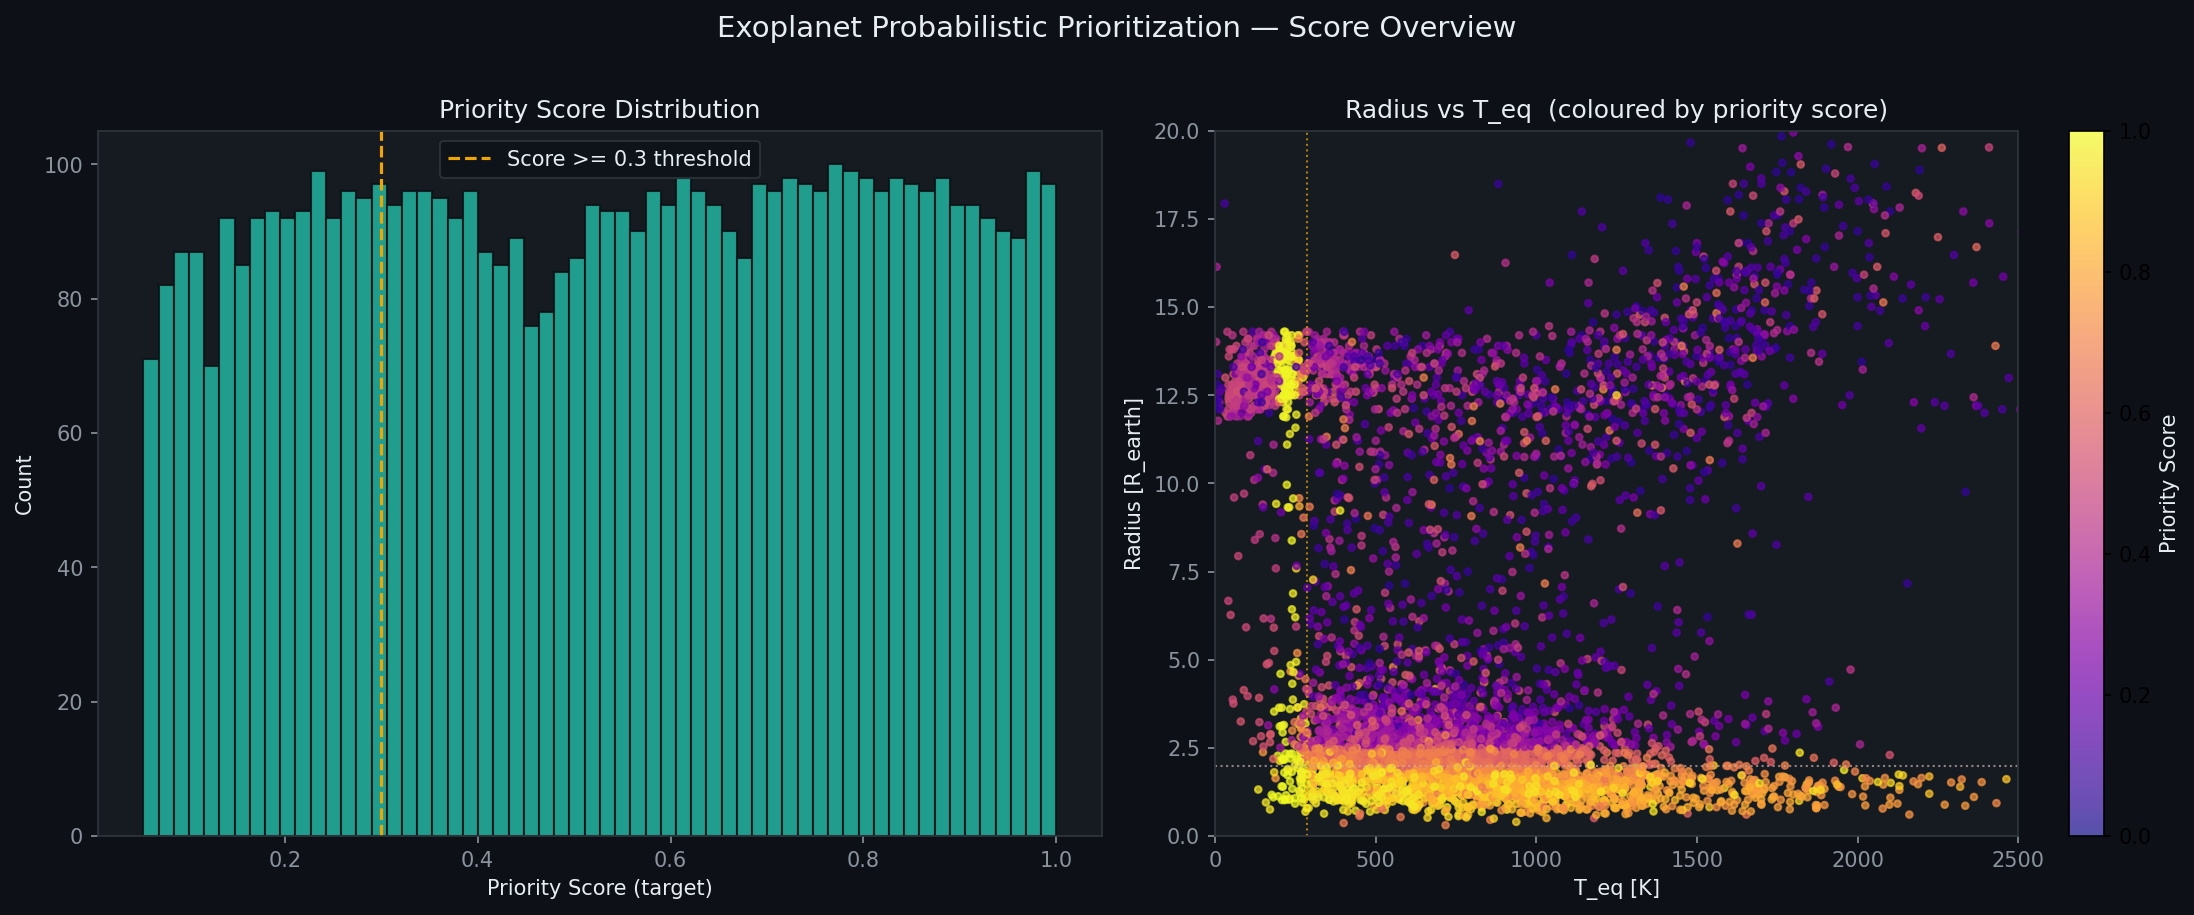
\includegraphics[width=0.85\textwidth]{../plots/priority_score_distribution.png}
\caption{Priority score distribution. Left: Histogram displaying the uniform distribution after quantile normalization. Right: Radius vs.\ equilibrium temperature scatter plot colored by priority score. Target planets cluster around $T_{\text{eq}} \approx 288\,\text{K}$ and $R_p \leq 2\,R_\oplus$.}
\label{fig:priority_dist}
\end{figure}

This uniform calibration:
\begin{enumerate}
    \item Maximizes the contrast between targets for ranking models.
    \item Prevents gradient saturation at the boundaries ($0$ or $1$) during training.
    \item Ensures the target behaves as a smooth, linear utility metric directly suitable for scheduling.
\end{enumerate}

\subsection{Label--Feature Overlap}

The priority label is a deterministic function of catalog columns (Appendix~\ref{app:priority}). Derived scores $f_{\text{thermal}}$, $f_{\text{esi}}$, and $f_{\text{rocky}}$ are not passed to the regressors. Their inputs are. Table~\ref{tab:leakage} records that overlap; it does not assert a no-leakage guarantee.

\begin{table}[H]
\centering
\caption{Label construction versus ML features. Derived scores are held out; the physical columns that define them are not.}
\label{tab:leakage}
\begin{tabular}{lcc}
\toprule
Quantity & Enters $P_{\text{astro}}$ / $D$ blend & In $\mathbf{X}$ (31 features) \\
\midrule
HZ factor $f_{\text{thermal}}$ (derived) & yes & no \\
ESI $E$ (derived) & yes & no \\
Rocky proxy $f_{\text{rocky}}$ (derived) & yes & no \\
\midrule
$R_p$, $\rho_p$ (rocky proxy and ESI) & yes & yes \\
$T_{\text{eq}}$ (ESI) & yes & yes \\
$F_{\text{insol}}$ (correlated with HZ / $T_{\text{eq}}$) & no (direct) & yes \\
$a$, $T_{\text{eff}}$, $L_\star$ (HZ geometry) & yes & yes \\
$e$, [Fe/H], age (diversity nudges) & yes & yes \\
Detectability $D$ ($15\%$ blend) & yes & yes \\
\bottomrule
\end{tabular}
\end{table}

Stage~1 therefore tests whether tree ensembles recover a physically motivated composite index from correlated catalog features. MAP@50 $= 1.000$ and RMSE $\approx 0.047$ on a $[0,1]$ target are the expected signature of that design, not evidence that the model learned astrophysics from independent observables. SHAP attributions (Section~\ref{sec:results}) rank $T_{\text{eq}}$, $T_{\text{eff}}$, $a$, and $R_p$ highest---the same quantities that define the label. A stricter hold-out of $\{R_p, \rho_p, T_{\text{eq}}, F_{\text{insol}}\}$ is implemented as \texttt{STRICT\_HOLDOUT\_FEATURES} in the code; that ablation is the appropriate test of ranking from remaining observables and is not the experiment reported in Table~\ref{tab:ml_results}.

Figure~\ref{fig:correlations} shows correlations among catalog columns. It does not demonstrate independence of $\mathbf{X}$ from the label.

\begin{figure}[H]
\centering
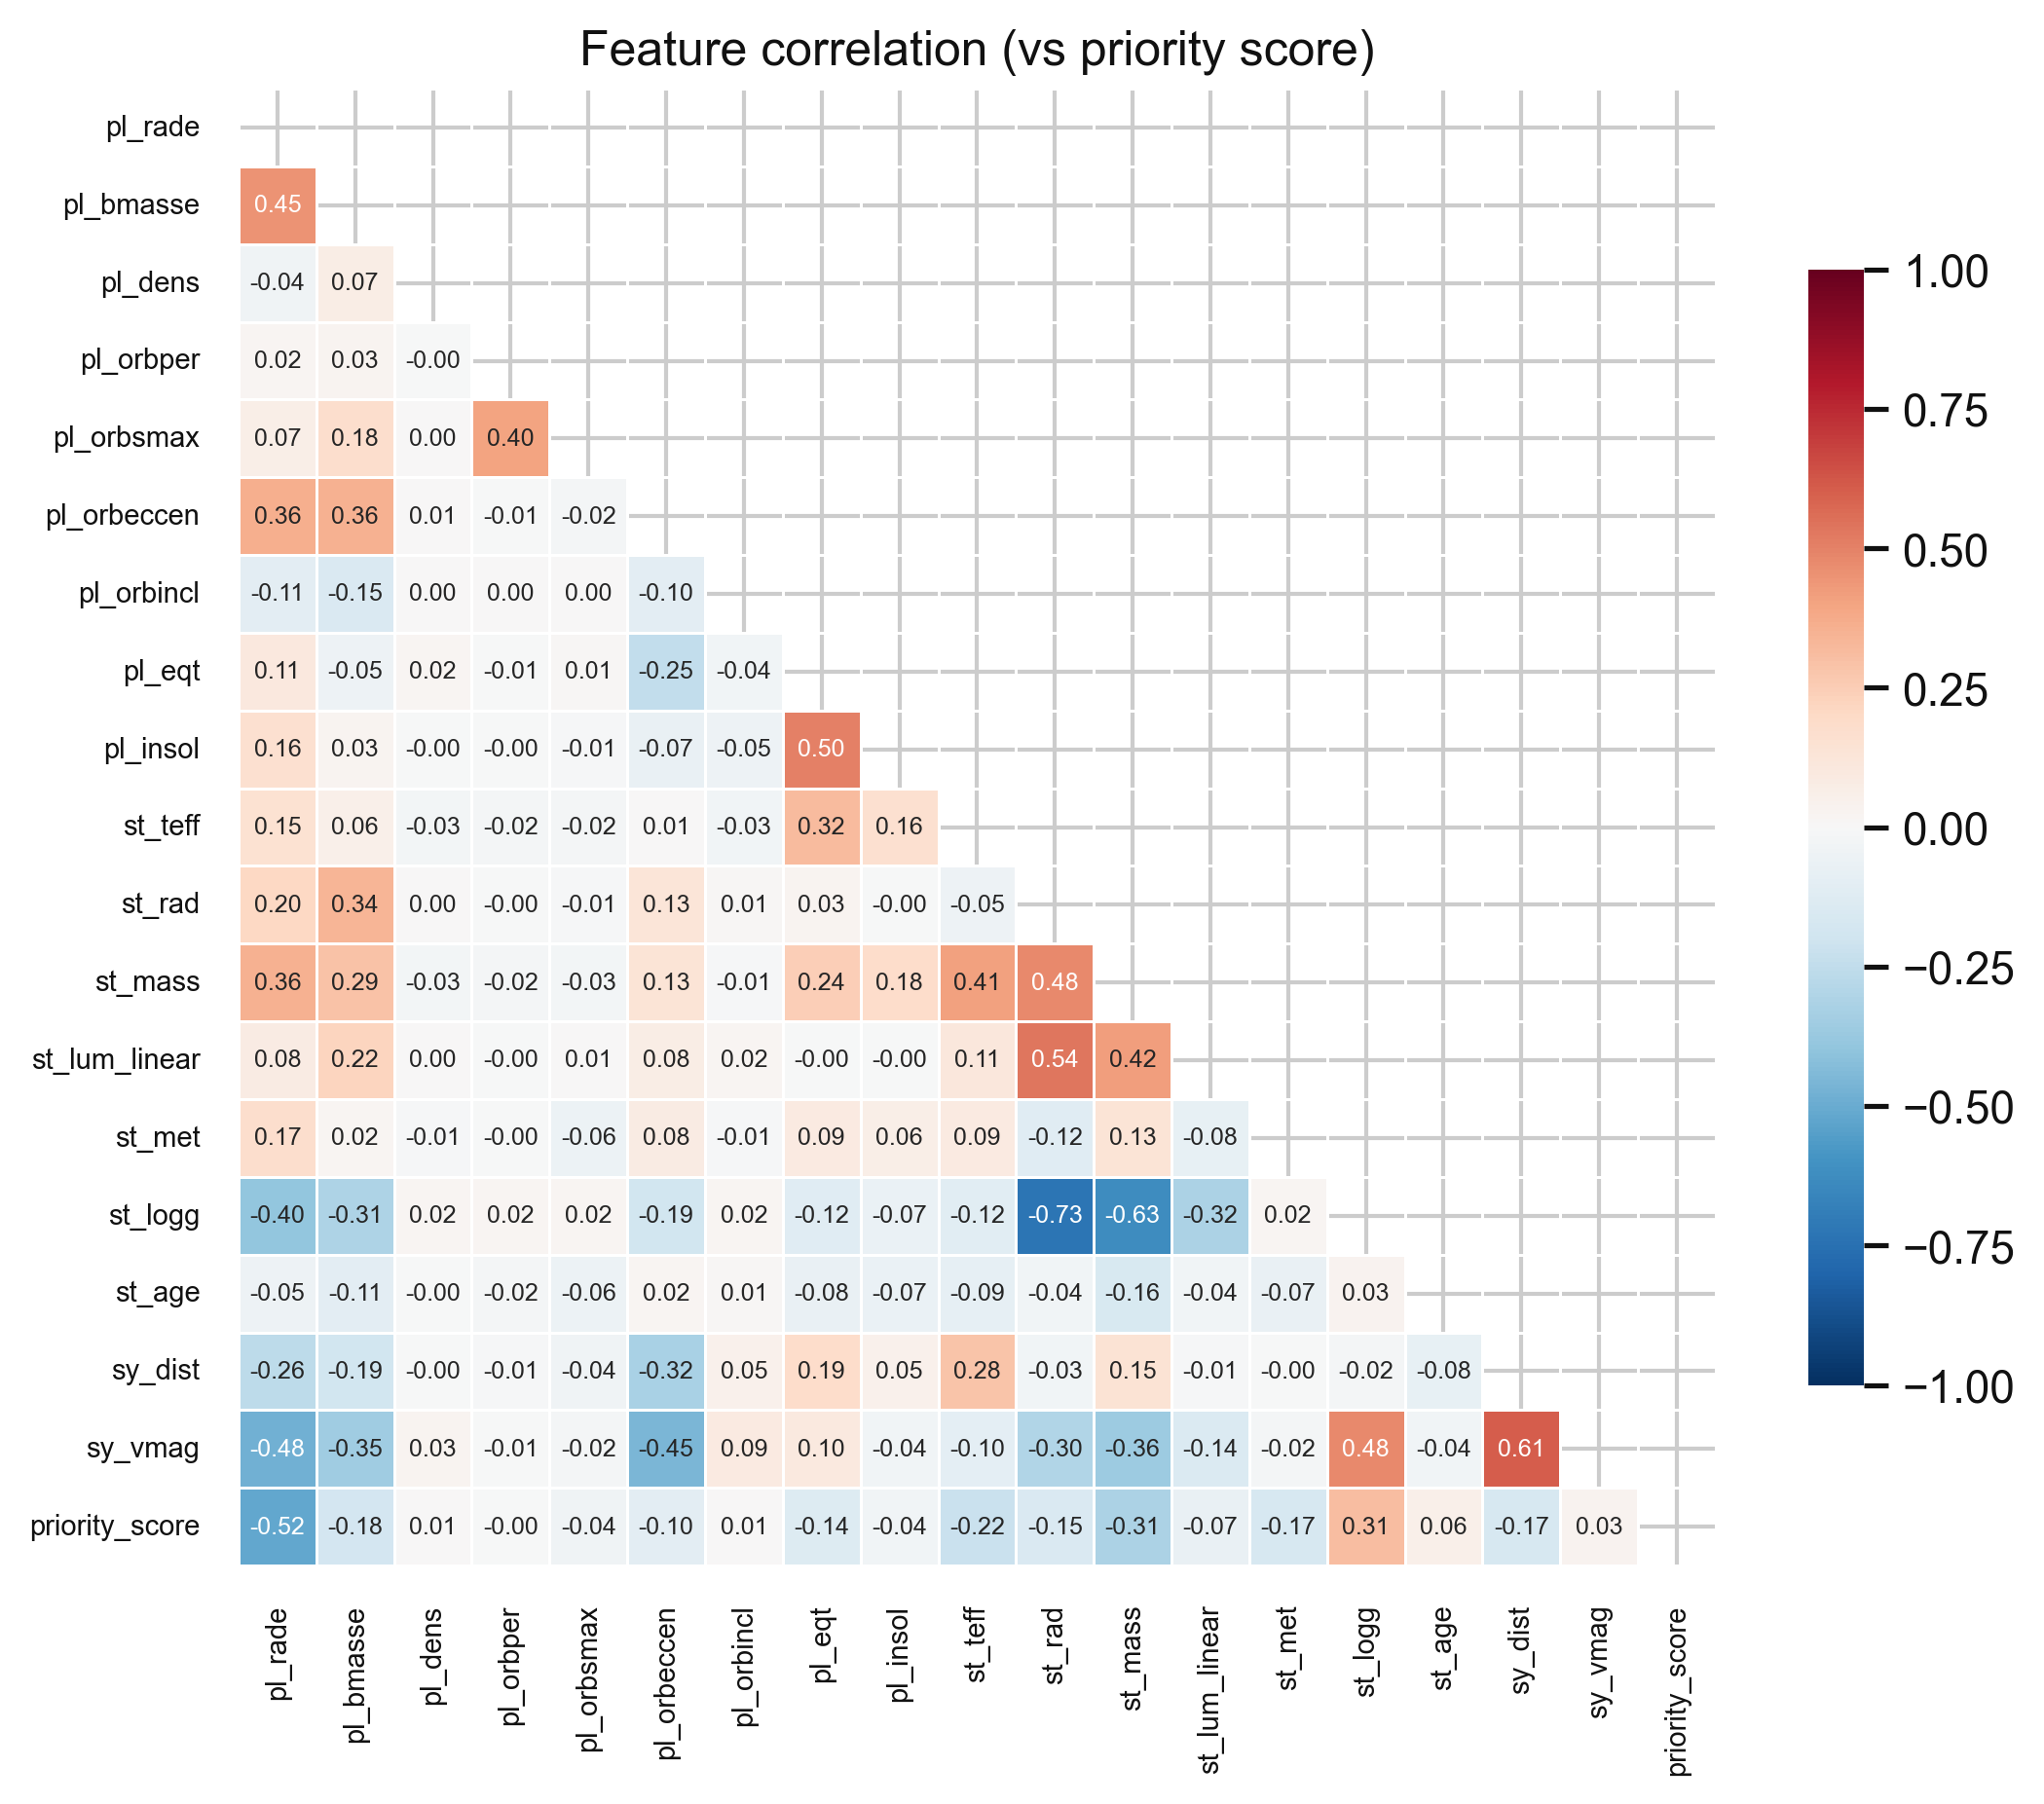
\includegraphics[width=0.65\textwidth]{../plots/feature_correlations.png}
\caption{Feature correlation matrix among catalog columns used as ML inputs. Physical correlations (e.g., $T_{\text{eq}}$ with $a$) are expected. This figure does not establish independence between features and the priority label.}
\label{fig:correlations}
\end{figure}

\subsection{Theoretical Justification of Utility Weights and Blends}
\label{sec:theory_weights}

A critical aspect of our framework is the selection of exponents in the continuous priority score (Eq.~\ref{eq:smoothed_mult}), the diversity nudge coefficients (Eq.~\ref{eq:nudge}), and the Composite Campaign Score weights (Eq.~\ref{eq:composite_score}). While these parameters might appear heuristic at first glance, they can be rigorously justified under Bayesian decision theory, multi-objective optimization, and Multi-Attribute Utility Theory (MAUT).

\paragraph{1. Dirichlet Prior Interpretation of the Astro-Utility Exponents.}
The exponents $(0.5, 0.3, 0.2)$ in our smoothed multiplicative joint utility (Eq.~\ref{eq:smoothed_mult}) represent the relative physical constraints of liquid water, solid surface, and bulk similarity, respectively. In a Bayesian setting, this joint utility can be interpreted as a prior probability distribution over scientific interest. By taking the logarithm, we obtain:
\begin{equation}
\log P_{\text{astro}} = 0.5 \log(H + \varepsilon) + 0.3 \log(R + \varepsilon) + 0.2 \log(E + \varepsilon)
\label{eq:dirichlet_log}
\end{equation}
Equation~\ref{eq:dirichlet_log} is mathematically isomorphic to a Dirichlet-distributed log-likelihood where the exponents function as concentration parameters (conjugate priors). This specific prior is chosen to reflect astrophysical consensus: liquid water stability ($H$) is the absolute prerequisite (highest weight 0.5), rocky composition ($R$) is secondary (weight 0.3), and bulk Earth-similarity ($E$) is tertiary (weight 0.2). The additive smoothing prior $\varepsilon = 0.1$ acts as a Laplacian-like regularization to prevent zero-frequency collapse, ensuring that borderline targets maintain positive probability support under the prior.

\paragraph{2. Diversity Nudges as Entropy Regularization.}
The secondary diversity nudges (Eq.~\ref{eq:nudge}) scale to a maximum contribution of $0.05$. This can be formally justified as a form of \textbf{entropy regularization} over the target selection policy. In active exploration, selecting only the highest-scoring target is sub-optimal if those targets are highly redundant (e.g., repeating observations of planets in the same stellar system). Adding small, bounded nudges for eccentricity ($f_{\text{ecc}}$), metallicity ($f_{\text{met}}$), and stellar age ($f_{\text{age}}$) acts as a regularization penalty:
\begin{equation}
U_{\text{regularized}}(p_i) = P_{\text{astro}}(p_i) + \lambda \mathcal{H}(p_i)
\label{eq:entropy_reg}
\end{equation}
where $\mathcal{H}(p_i)$ is the target-specific diversity vector, and $\lambda = 0.05$ is the regularization strength. This is mathematically equivalent to Kullback-Leibler (KL) regularization in reinforcement learning, which prevents the policy from collapsing into a singular delta-distribution and forces exploration across the physical parameter space.

\paragraph{3. Multi-Attribute Utility Theory (MAUT) and the Pareto Frontier.}
The Composite Campaign Score weights $(0.35, 0.25, 0.20, 0.20)$ in Eq.~\ref{eq:composite_score} map directly to MAUT, which establishes that any multi-objective decision problem under constraints can be resolved by maximizing a weighted additive combination of individual utility functions, provided the objectives satisfy mutual utility independence.

Furthermore, these weights define a specific vector in the multi-objective space that projects onto the non-dominated \textbf{Pareto-optimal frontier}. We select these specific weights to balance three competing dimensions:
\begin{itemize}
    \item \textbf{Astrophysical Merit} ($0.35 \cdot G_{\text{norm}}$ and $0.20 \cdot P_{\text{norm}}$): Dedicated to prioritizing high-habitability, high-interest targets.
    \item \textbf{Observation Efficiency} ($0.20 \cdot E_{\text{norm}}$): Safeguarding the campaign against wasting telescope hours under bad weather.
    \item \textbf{Scientific Diversity} ($0.25 \cdot D_{\text{norm}}$): Ensuring that observations are distributed across a broad physical parameter space.
\end{itemize}
While these weights are fixed in our primary evaluation, our framework's sequential decision structure is fully compatible with dynamic weight elicitation. Future work can implement \textbf{Bayesian preference elicitation} or \textbf{Inverse Reinforcement Learning (IRL)} to dynamically learn these weights from real-world astronomical schedules, allowing the system to match the subjective preferences of different scientific committees.

%% ============================================================
\section{Catalog-Index Recovery via Tree Ensembles}
\label{sec:ml}

\subsection{Data Acquisition and Imputation}

Data are obtained from the Planetary Systems Composite Parameters (\texttt{pscomppars}) table of the NASA Exoplanet Archive using TAP ADQL queries \cite{nasa_archive}. The query used in this repository returned 6{,}284 records. The catalog was frozen on 2026-05-26; the live archive changes, so a later query will not reproduce this row count. The ADQL is given in Appendix~\ref{app:adql}.

Where physical parameters are missing, we perform scientifically grounded imputations:
\begin{itemize}
    \item Missing planetary masses are imputed using the empirical mass-radius relations of Chen \& Kipping (2017) \cite{chen2017}:
    \begin{equation}
    M_p = \begin{cases}
    0.9718\, R_p^{3.58} & R_p \leq 1.23\,R_\oplus \\
    1.436\, R_p^{1.70}  & 1.23 < R_p \leq 14.26\,R_\oplus
    \end{cases}
    \label{eq:chen_kipping}
    \end{equation}
    \item Missing equilibrium temperatures ($T_{\text{eq}}$) are derived from stellar parameters via the Stefan-Boltzmann relation assuming a Bond albedo $A_B = 0.3$:
    \begin{equation}
    T_{\text{eq}} = T_{\text{eff}} \cdot \sqrt{\frac{R_\star}{2a}} \cdot (1 - A_B)^{1/4}
    \label{eq:teq_calc}
    \end{equation}
\end{itemize}
After filtering and cleaning, we obtain $5{,}522$ planets and 31 catalog features (Appendix~\ref{app:features}). Those features include the physical columns that define the label (Table~\ref{tab:leakage}).

\subsection{Observation Feasibility Analysis}

Telescope observability is modeled as a first-class predictive feature. We display the distribution of physical observability parameters (composite SNR, distance penalties, and detectability blends) in Figure~\ref{fig:observability}.

\begin{figure}[H]
\centering
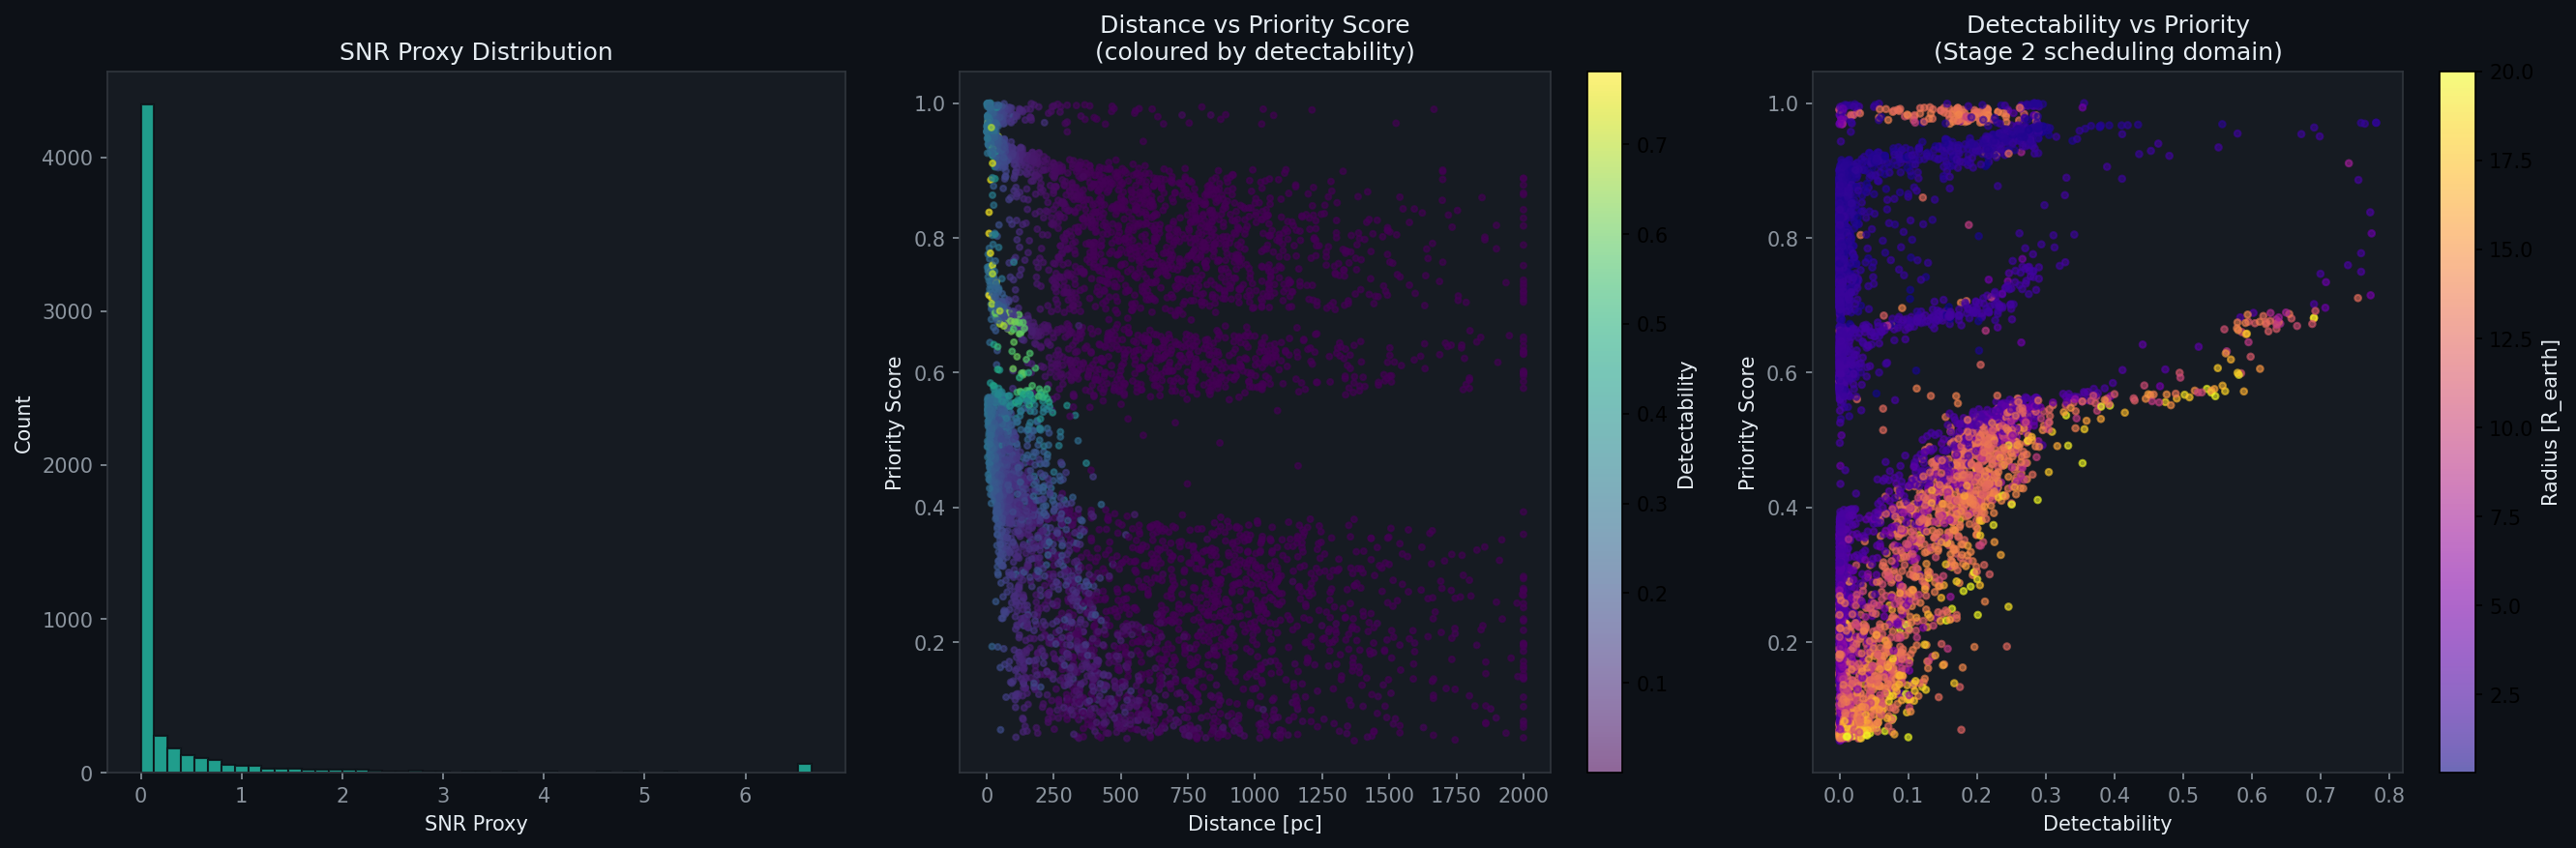
\includegraphics[width=0.85\textwidth]{../plots/observability_analysis.png}
\caption{Observation feasibility analysis. Left: Distribution of the transit spectroscopic SNR proxy. Center: Apparent system distance vs.\ priority score colored by detectability (nearby high-priority planets represent high-value targets). Right: Composite detectability vs.\ priority score, establishing the domain for scheduler campaigns.}
\label{fig:observability}
\end{figure}

\subsection{Predictive Models}

We train four tree-based ensemble regression models to map the 31-dimensional feature matrix $\mathbf{X} \in \mathbb{R}^{n \times p}$ to the quantile-normalized priority scores $\mathbf{y} \in [0,1]^n$. The hyperparameters for the four classifiers (Random Forest, XGBoost, GBR, and LightGBM) are detailed in Appendix C.

Ensemble trees are uniquely robust in this domain. Unlike linear regressors or neural networks, decision trees make no prior assumptions about the shape of the data and are insensitive to multi-modal distributions (such as the distinct clusters formed by gaseous sub-Neptunes vs.\ rocky super-Earths in radius-density space).

\subsection{Ranking-Aware Evaluation Metrics}

While the models are trained using Mean Squared Error (MSE) loss, our primary scientific objective is to establish an optimal \textit{ranking} of planets. We therefore evaluate the models using ranking-appropriate metrics:

\subsubsection{Normalized Discounted Cumulative Gain (NDCG@K)}
\begin{equation}
\text{NDCG@K} = \frac{\text{DCG@K}}{\text{IDCG@K}}, \qquad \text{DCG@K} = \sum_{i=1}^{K} \frac{y_{\pi(i)}}{\log_2(i+1)}
\label{eq:ndcg}
\end{equation}
where $\pi(i)$ represents the index of the planet ranked at position $i$ by the model's predicted scores, and IDCG is the ideal (oracle) DCG. NDCG@K rewards models that place high-priority targets at the very top of the ranking, applying a logarithmic discount at lower ranks.

\subsubsection{Mean Average Precision (MAP@K)}
\begin{equation}
\text{MAP@K} = \frac{\sum_{k=1}^{K} P@k \cdot \mathbf{1}[y_{\pi(k)} \geq \theta]}{|\{i : y_i \geq \theta\}|}
\label{eq:map}
\end{equation}
where $\theta = 0.70$ is the high-priority relevance threshold and $P@k$ is precision at rank $k$.

\subsubsection{Spearman Rank Correlation ($\rho_s$) and Kendall's Tau ($\tau$)}
We compute the rank correlation metrics to evaluate the monotonic alignment between predicted priorities and true priorities across the entire population \cite{spearman1904, kendall1938}.

\subsubsection{Regret@K}
\begin{equation}
\text{Regret@K} = 1 - \frac{\sum_{i \in \hat{\mathcal{T}}_K} y_i}{\sum_{i \in \mathcal{T}_K^*} y_i}
\label{eq:regret}
\end{equation}
where $\hat{\mathcal{T}}_K$ represents the top-$K$ targets selected by the model and $\mathcal{T}_K^*$ represents the ideal top-$K$ oracle targets. Regret@K measures the percentage of maximum possible scientific utility missed by using the model's recommendations.

\subsection{Epistemic Uncertainty Quantification}

For the Random Forest model, we estimate the epistemic prediction uncertainty $\hat{\sigma}_i$ for each planet $i$ as the standard deviation across individual tree predictions:
\begin{equation}
\hat{\mu}_i = \frac{1}{M}\sum_{m=1}^{M} h_m(\mathbf{x}_i), \qquad \hat{\sigma}_i = \sqrt{\frac{1}{M}\sum_{m=1}^{M}(h_m(\mathbf{x}_i) - \hat{\mu}_i)^2}
\label{eq:tree_var}
\end{equation}
where $h_m$ represents the $m$-th decision tree in the ensemble, and $M = 300$.

\subsection{Scientific Gain Heuristic}

We treat $\hat{\sigma}_i$ as a scheduling exploration bonus, not as Shannon entropy of an atmospheric retrieval. We define Scientific Gain of observing target $i$ as:
\begin{equation}
\text{SG}_i = \hat{\sigma}_i \times D_i
\label{eq:scigain}
\end{equation}
which represents the expected reduction in epistemic entropy scaled by the expected information extraction efficiency $D_i$ (detectability) per telescope hour. This operationalizes the core active learning principle: \textit{schedule observations where you will learn the most per telescope hour}. Figure~\ref{fig:uncertainty} displays the relationship between predicted priority, tree variance, and the resulting top-20 scientific gain targets.

\begin{figure}[H]
\centering
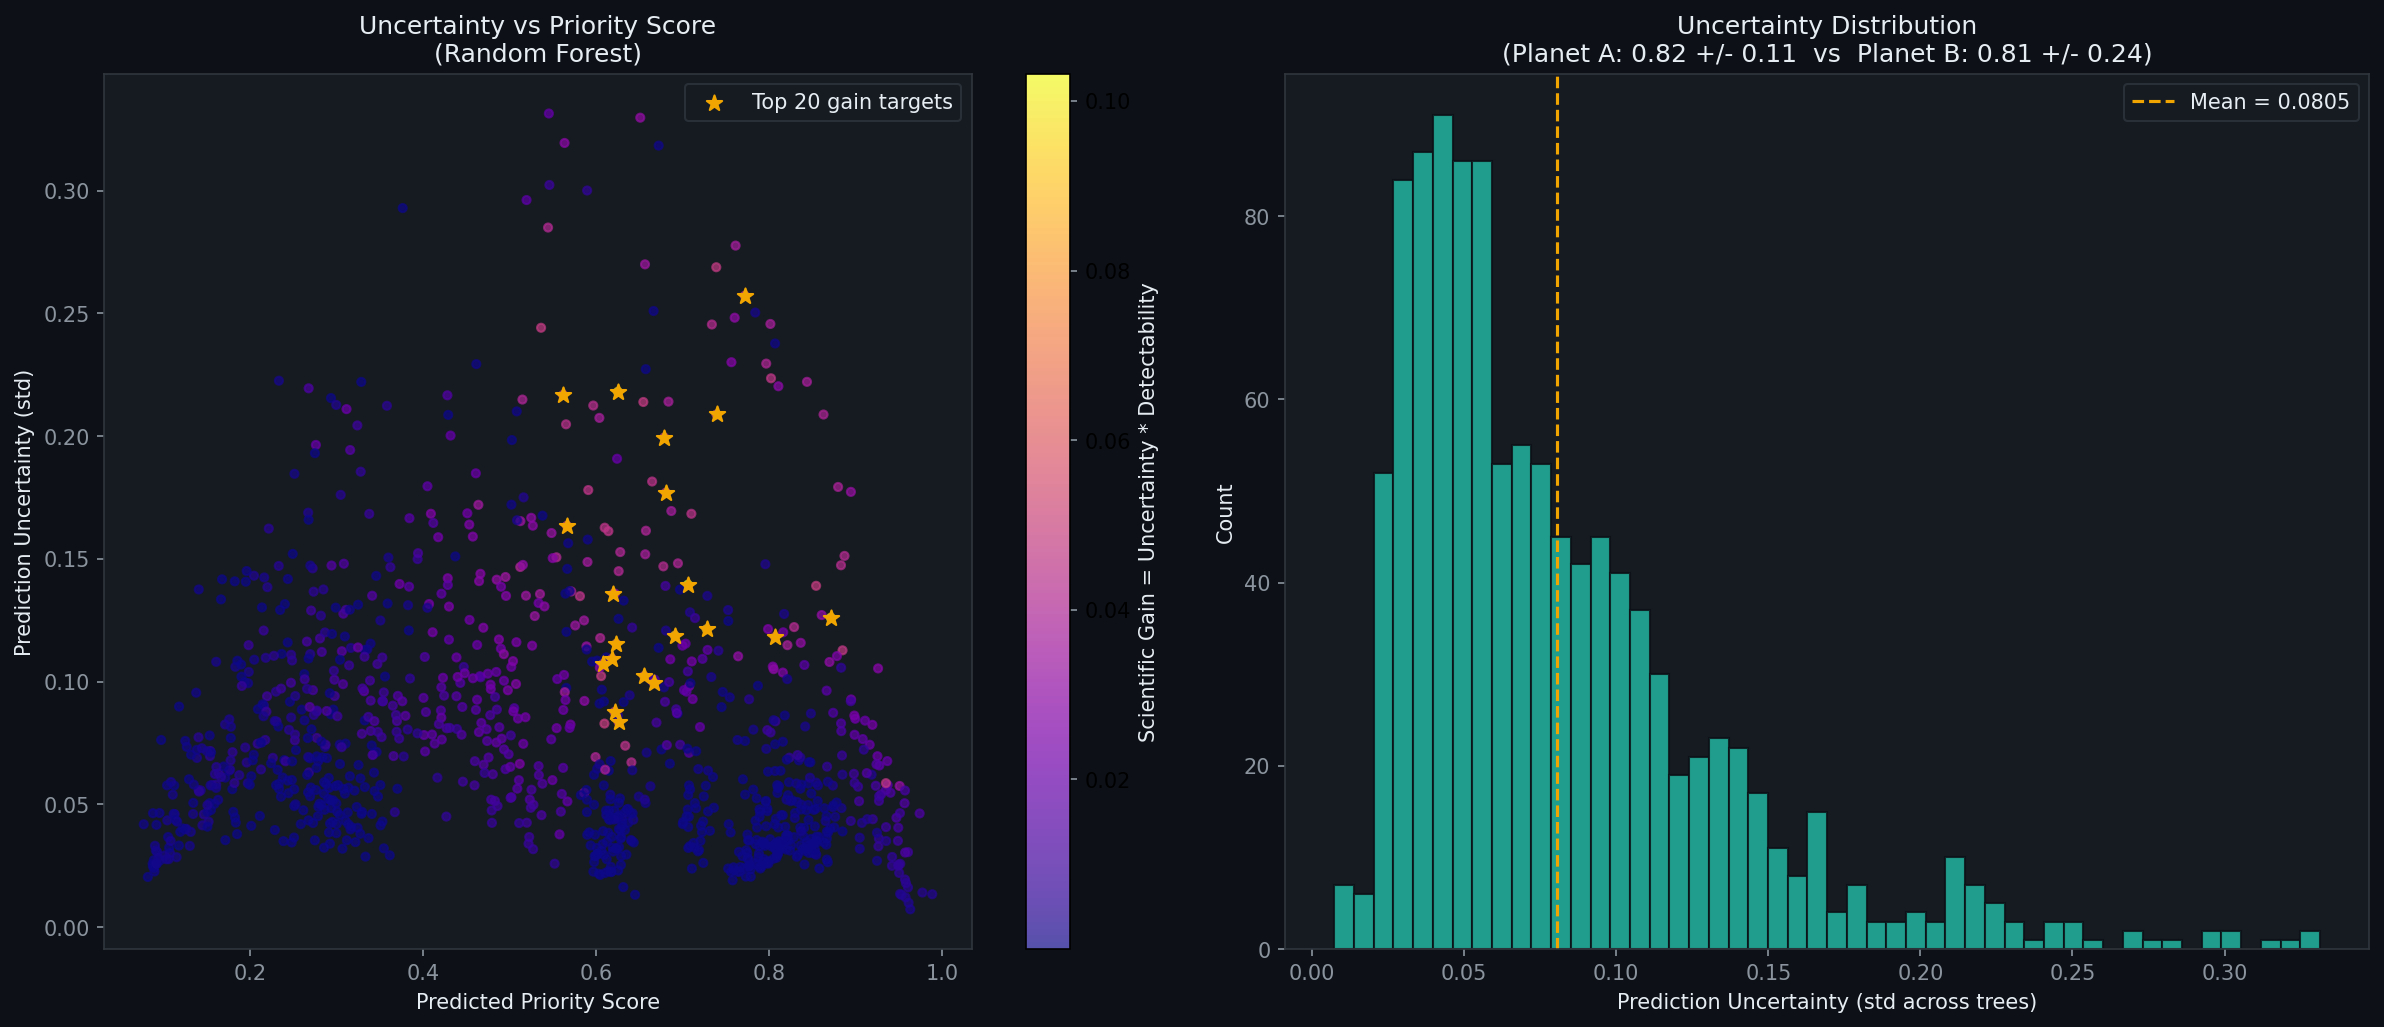
\includegraphics[width=0.85\textwidth]{../plots/uncertainty_analysis.png}
\caption{Active target profiling analysis. Left: Estimated prediction uncertainty ($\hat{\sigma}$) vs.\ predicted priority ($\hat{\mu}$), colored by Scientific Gain. Gold stars mark the top-20 active survey targets. Right: Empirical distribution of prediction uncertainty (std across tree predictions) across the candidate population.}
\label{fig:uncertainty}
\end{figure}

%% ============================================================
\section{Simulated Campaign Scheduler}
\label{sec:scheduler}

Transitioning from a static prioritization list to an active observation campaign requires an operational scheduler that satisfies the environmental and physical constraints outlined in Section~\ref{sec:problem}.

\subsection{Operational Constraints and Cost Modeling}

At round $t$, target scheduling is limited by:
\begin{enumerate}
    \item \textbf{Target Visibility ($V_i^{(t)} \in \{0, 1\}$):} Constraining observations to planets visible during the current pointing window.
    \item \textbf{Integration Exposure Cost ($C_i^{(t)}$):} We model the telescope integration cost (in hours) as:
    \begin{equation}
    C_i^{(t)} = \frac{C_{i,\text{static}}}{W^{(t)} + 10^{-6}}
    \label{eq:cost_model}
    \end{equation}
    where $C_{i,\text{static}}$ represents the static baseline integration time dictated by the target's J-band magnitude, system distance, and transit duration:
    \begin{equation}
    C_{i,\text{static}} = C_{\text{base}} + \text{clip}\left(0.15(J_i - 8), 0, 2.0\right) + \text{clip}\left(0.3 \log\left(1 + \frac{d_i}{50\,\text{pc}}\right), 0, 1.5\right) + \frac{T_{\text{dur}, i}}{24.0}
    \label{eq:static_cost}
    \end{equation}
    where $C_{\text{base}} = 0.5$ hours and the cost is capped at $4.0$ hours. Equation~\ref{eq:cost_model} establishes that bad weather ($W^{(t)} \to 0$) exponentially increases integration times, reducing the number of targets the telescope can observe within its round budget $B^{(t)} = 8.0$ hours. Figure~\ref{fig:weather_seq} displays the time-varying environmental quality sequence used in the campaign simulations.
\end{enumerate}

\begin{figure}[H]
\centering
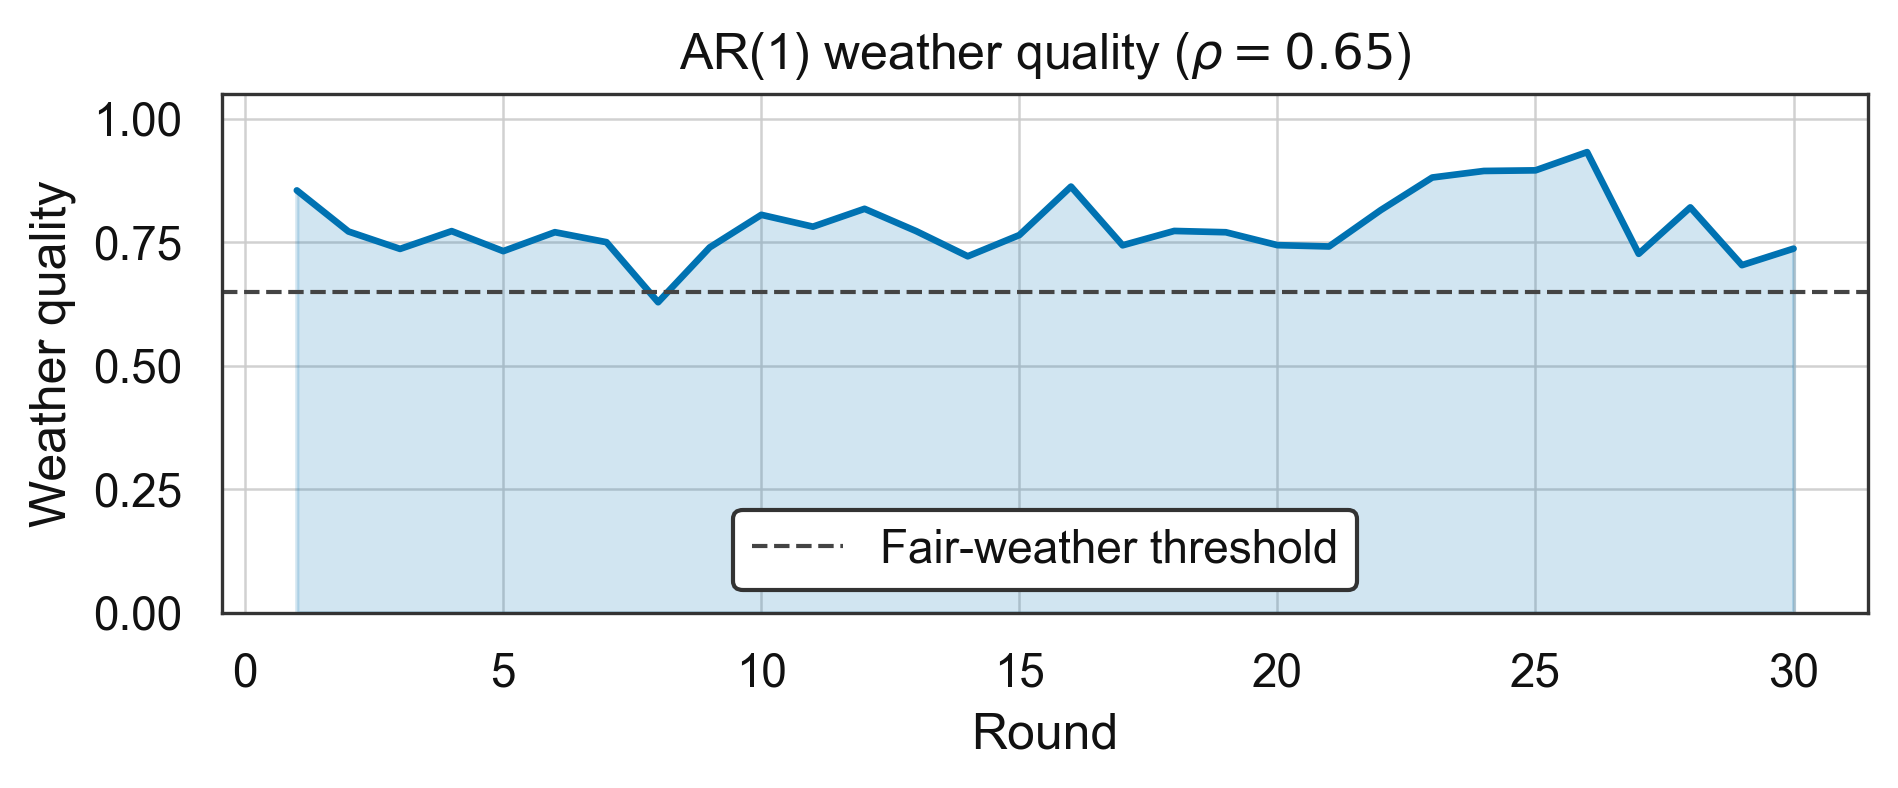
\includegraphics[width=0.75\textwidth]{../plots/s2_weather_sequence.png}
\caption{Generated AR(1) weather and visibility quality sequence over 30 rounds ($\rho = 0.65$), defining the dynamic time-varying campaign environment constraint.}
\label{fig:weather_seq}
\end{figure}

\subsection{The Dynamic Schedulers}

We simulate and compare five operational schedulers over a 30-round campaign:
\begin{enumerate}
    \item \textbf{Oracle Scheduler (same-objective upper bound):} Replaces $\hat{\mu}_i$ in Eq.~\ref{eq:utility_decomp} with the ground-truth priority $P_i^{\text{true}}$ and otherwise uses the same utility, constraints, and greedy selection as the Adaptive Scheduler. It is a perfect-knowledge implementation of the \emph{same} objective, not an independent scientific benchmark. Near-Oracle composite scores mainly show that the heuristic tracks that objective.
    \item \textbf{Adaptive Scheduler (Proposed):} Employs the predicted priority mean $\hat{\mu}_i$, predicted epistemic uncertainty $\hat{\sigma}_i$, and detectability $D_i$ inside the active utility function (Eq.~\ref{eq:utility_decomp}). It dynamically updates the target database at each round, reducing the uncertainty $\hat{\sigma}_i$ of observed targets by half upon completion of an observation. It uses the exponential weight decay schedule (Eq.~\ref{eq:decay}) to transition from active exploration to exploitation (Figure~\ref{fig:weight_decay}).
    \item \textbf{Detectability Greedy (Baseline):} A single-objective baseline that schedules visible targets prioritizing only their physical detectability $D_i$, maximizing the number of observed targets regardless of their habitability or scientific interest.
    \item \textbf{Static Priority (Baseline):} Schedules visible targets prioritizing only the predicted priority mean $\hat{\mu}_i$ (strict exploitation), without updating uncertainties or considering observational efficiency.
    \item \textbf{Uncertainty Greedy (Baseline):} Schedules targets prioritizing only the predicted uncertainty $\hat{\sigma}_i$ (strict exploration), attempting to reduce model variance without considering target priorities.
\end{enumerate}

\begin{figure}[H]
\centering
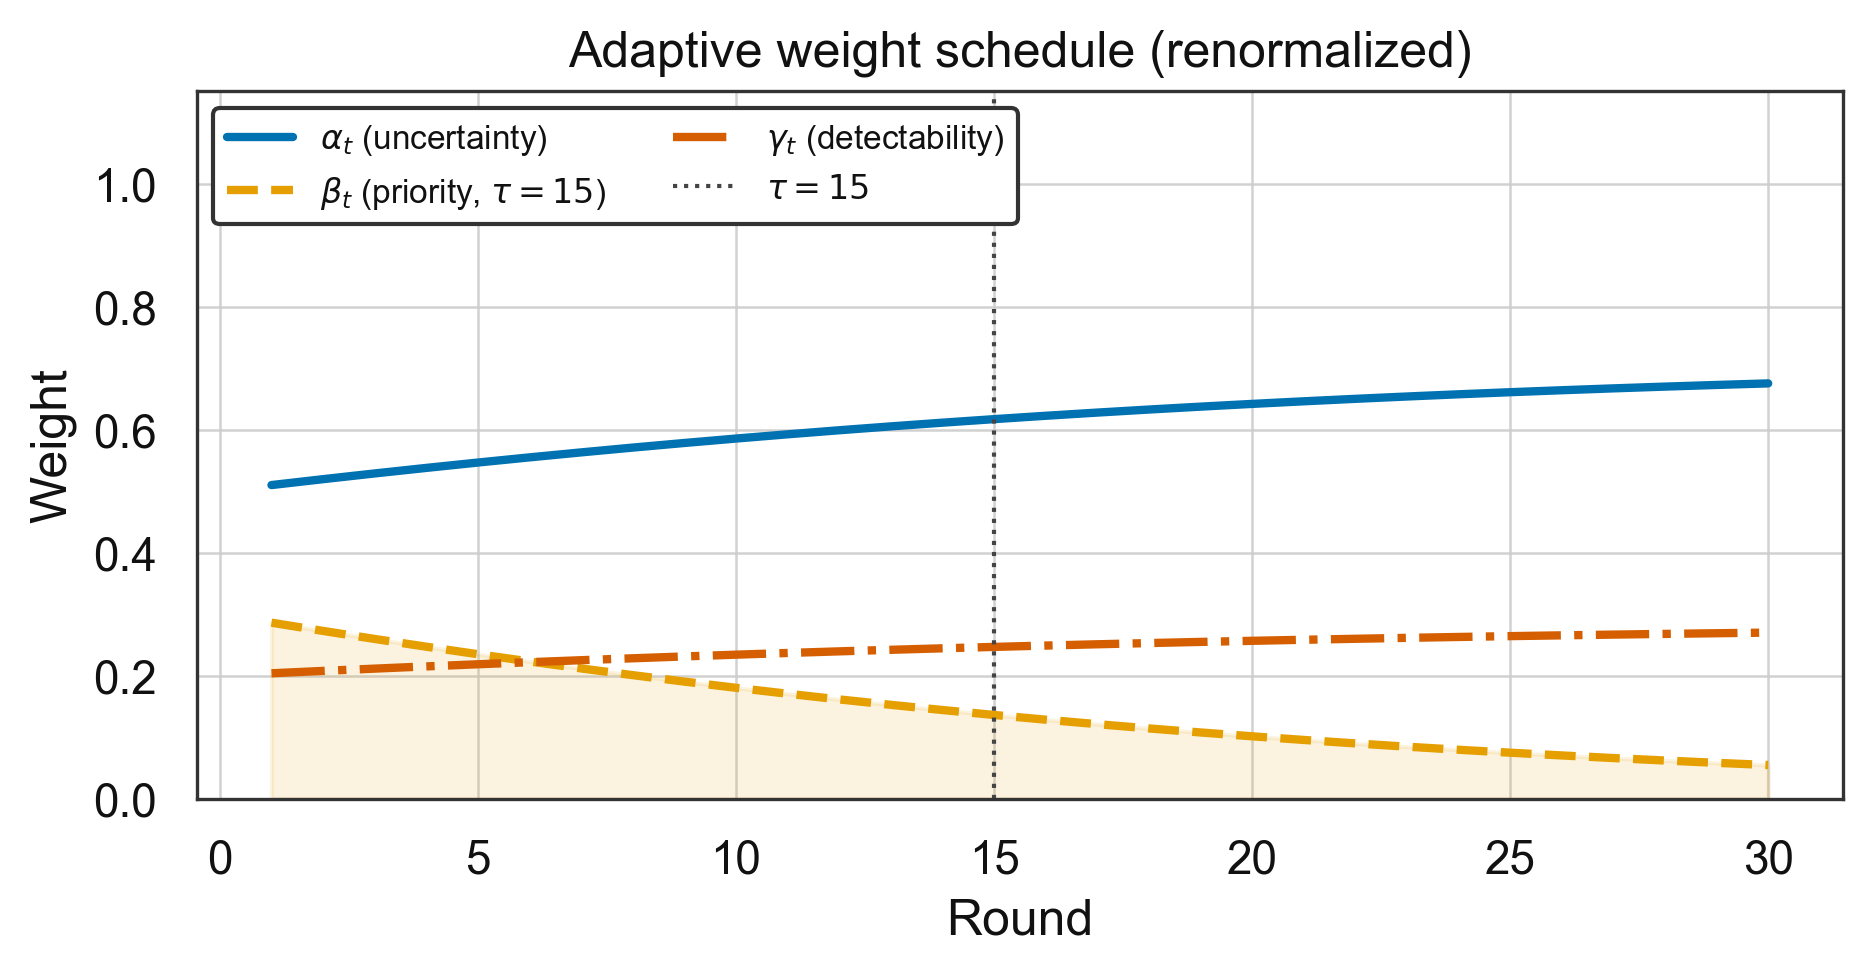
\includegraphics[width=0.75\textwidth]{../plots/s2_weight_decay.png}
\caption{Proposed Adaptive Scheduler: Dynamic exploration-exploitation weight decay schedule over 30 rounds ($\tau = 15.0$ rounds).}
\label{fig:weight_decay}
\end{figure}

For all schedulers, the target utility is scaled by operational efficiency:
\begin{equation}
\text{Utility}_i^{(t)} = \frac{\text{Gain}_i^{(t)} \cdot V_i^{(t)}}{C_i^{(t)}}
\label{eq:scheduler_utility}
\end{equation}
At each round, targets with the highest $\text{Utility}_i^{(t)}$ are greedily selected until the exposure budget $B^{(t)}$ is exhausted. This is a greedy knapsack-style heuristic: integration cost is the item weight, utility is the value, and $B^{(t)}$ is the capacity.

\subsection{Multi-Objective Campaign Score}

The composite score used for ranking schedulers is
\begin{equation}
\text{CompositeScore} = 0.35 \cdot G_{\text{norm}} + 0.25 \cdot D_{\text{norm}} + 0.20 \cdot E_{\text{norm}} + 0.20 \cdot P_{\text{norm}}
\label{eq:composite_score}
\end{equation}
where each component is normalized relative to the idealized reference scheduler:
\begin{itemize}
    \item $G_{\text{norm}} = G_{\text{scheduler}} / G_{\text{Oracle}}$: Normalized Cumulative Scientific Gain (total epistemic entropy reduction).
    \item $D_{\text{norm}} = \text{Diversity}_{\text{scheduler}} / \text{Diversity}_{\text{Oracle}}$: Normalized Campaign Parameter Space Coverage (measured via Shannon entropy across five planetary parameters: radius, semi-major axis, temperature, density, and eccentricity).
    \item $E_{\text{norm}} = E_{\text{scheduler}} / E_{\text{Oracle}}$: Normalized Observation Efficiency (scientific gain acquired per telescope hour).
    \item $P_{\text{norm}} = P_{\text{scheduler}} / P_{\text{Oracle}}$: Normalized Target Priority Coverage (mean true priority score of observed planets).
\end{itemize}
Under this formulation, the idealized Oracle obtains a score of exactly $100\%$, and all schedulers are graded on their percentage of idealized reference performance.

\subsection{Computational Complexity}
\label{sec:complexity}

Inference and per-round selection are intended to be cheap relative to a campaign simulation, not flight software.

\paragraph{Stage 1.}
A tree-ensemble forward pass scales as $\mathcal{O}(N \cdot M \cdot d)$ with $N$ planets, $M$ trees, and average depth $d$. We do not report wall-clock microbenchmarks: no CPU model, trial count, or variance was recorded.

\paragraph{Stage 2.}
Visibility and cost scans are $\mathcal{O}(N)$. Ranking a visible pool of size $N_{\text{vis}}$ is $\mathcal{O}(N_{\text{vis}} \log N_{\text{vis}})$, or $\mathcal{O}(N_{\text{vis}} \log K)$ if a size-$K$ heap is used. Exact MILP/TSPTW observatory schedulers (e.g., AstroQ \cite{lubin2026astroq}) solve a different problem and are not compared on runtime here.

%% ============================================================
\section{Empirical Results and Analysis}
\label{sec:results}

\subsection{Target Prioritization Accuracy}

We evaluate the four regressors on a held-out test set (80/20 split, \texttt{random\_state=42}) and 5-fold shuffled cross-validation (same seed). Table~\ref{tab:ml_results} reports catalog-index recovery, not ranking from independent observables.

\begin{table}[H]
\centering
\caption{Recovery of the constructed priority score from catalog features that overlap the label (test set). CV column is mean $\pm$ standard deviation across 5 folds, not a standard error of the mean. MAP@50 $= 1.000$ is expected under Table~\ref{tab:leakage}.}
\label{tab:ml_results}
\begin{tabular}{lcccccccc}
\toprule
Model & NDCG@50 & MAP@50 & Spearman $\rho$ & Kendall $\tau$ & Regret@50 & $R^2$ & RMSE & CV Spearman $\rho$ \\
\midrule
Random Forest     & 0.977 & 1.000 & 0.972 & 0.882 & 0.024 & 0.943 & 0.066 & $0.966 \pm 0.004$ \\
XGBoost           & 0.990 & 1.000 & 0.985 & 0.930 & 0.011 & 0.971 & 0.047 & $0.981 \pm 0.004$ \\
Gradient Boosting & 0.975 & 0.985 & 0.984 & 0.929 & 0.030 & 0.968 & 0.050 & $0.981 \pm 0.004$ \\
LightGBM          & \textbf{0.989} & \textbf{1.000} & \textbf{0.985} & \textbf{0.933} & \textbf{0.010} & \textbf{0.971} & \textbf{0.047} & $\mathbf{0.982 \pm 0.003}$ \\
\bottomrule
\end{tabular}
\end{table}

All four models achieve NDCG@50 $> 0.975$ and Spearman $\rho_s > 0.97$. That tightness, including CV standard deviations of $\pm 0.003$--$0.004$, is consistent with approximating a deterministic function of the inputs. LightGBM recovers 99\% of top-50 label mass (Regret@50 $= 0.010$). These numbers should not be read as a no-leakage generalization result. Figure~\ref{fig:ml_plots} shows the corresponding diagnostics.

\begin{figure}[H]
\centering
\begin{subfigure}[b]{0.32\textwidth}
    \centering
    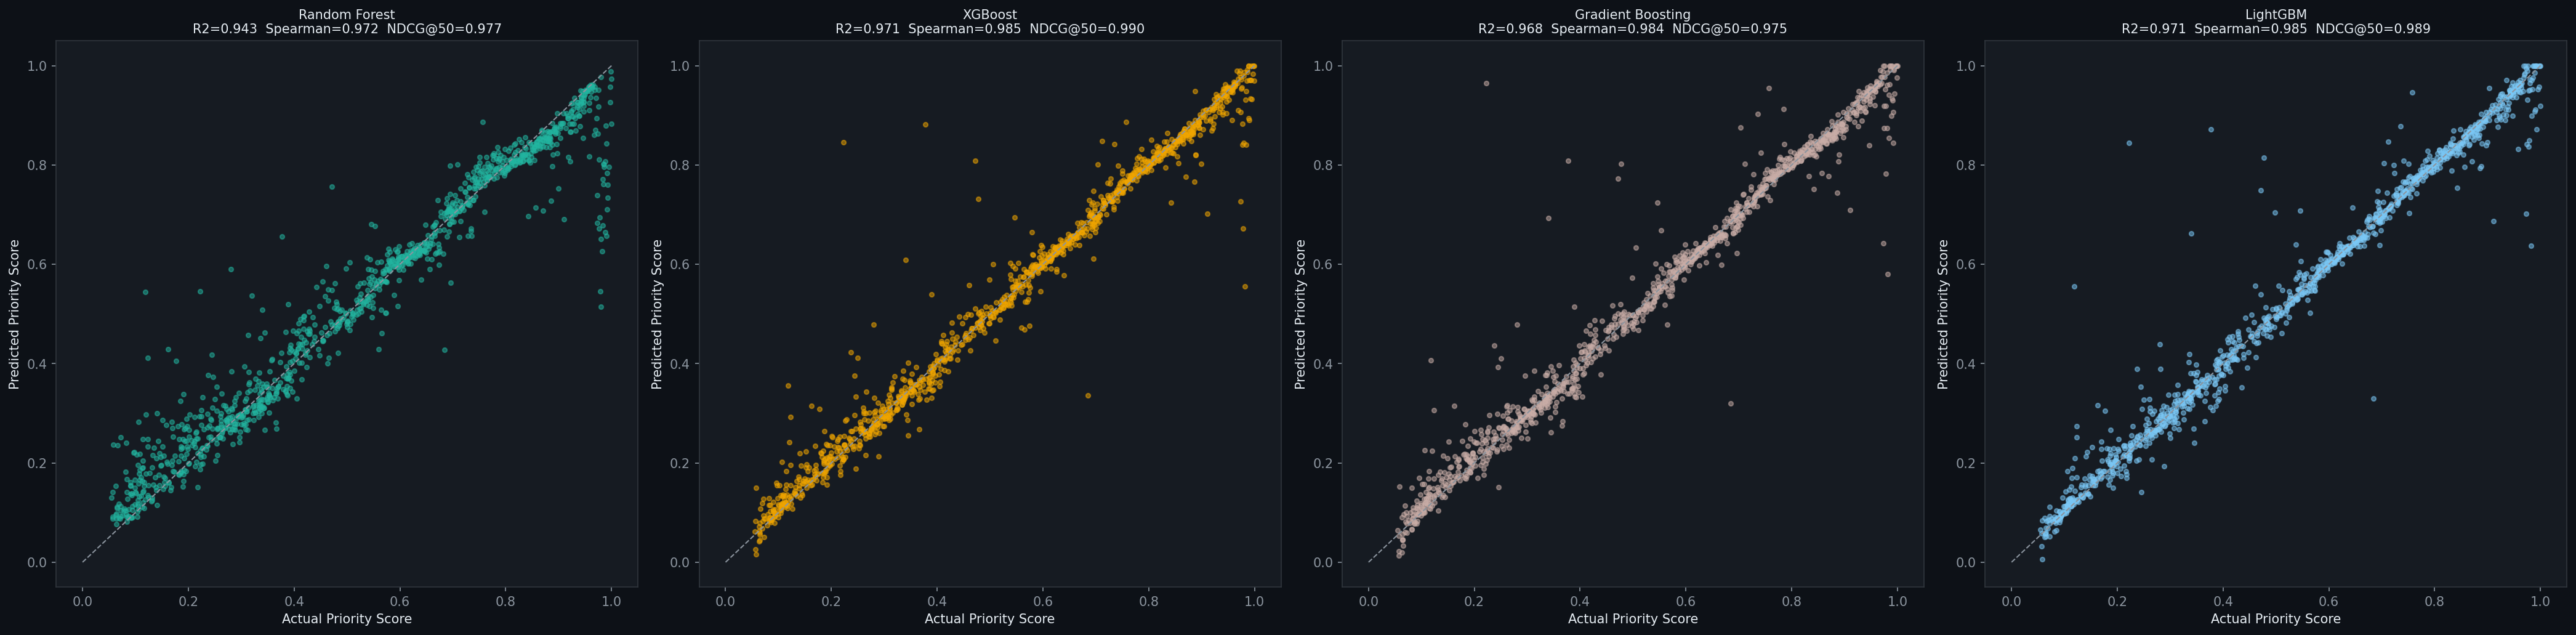
\includegraphics[width=\textwidth]{../plots/predicted_vs_actual.png}
    \caption{Predicted vs.\ Actual}
    \label{fig:pred_vs_actual}
\end{subfigure}
\hfill
\begin{subfigure}[b]{0.32\textwidth}
    \centering
    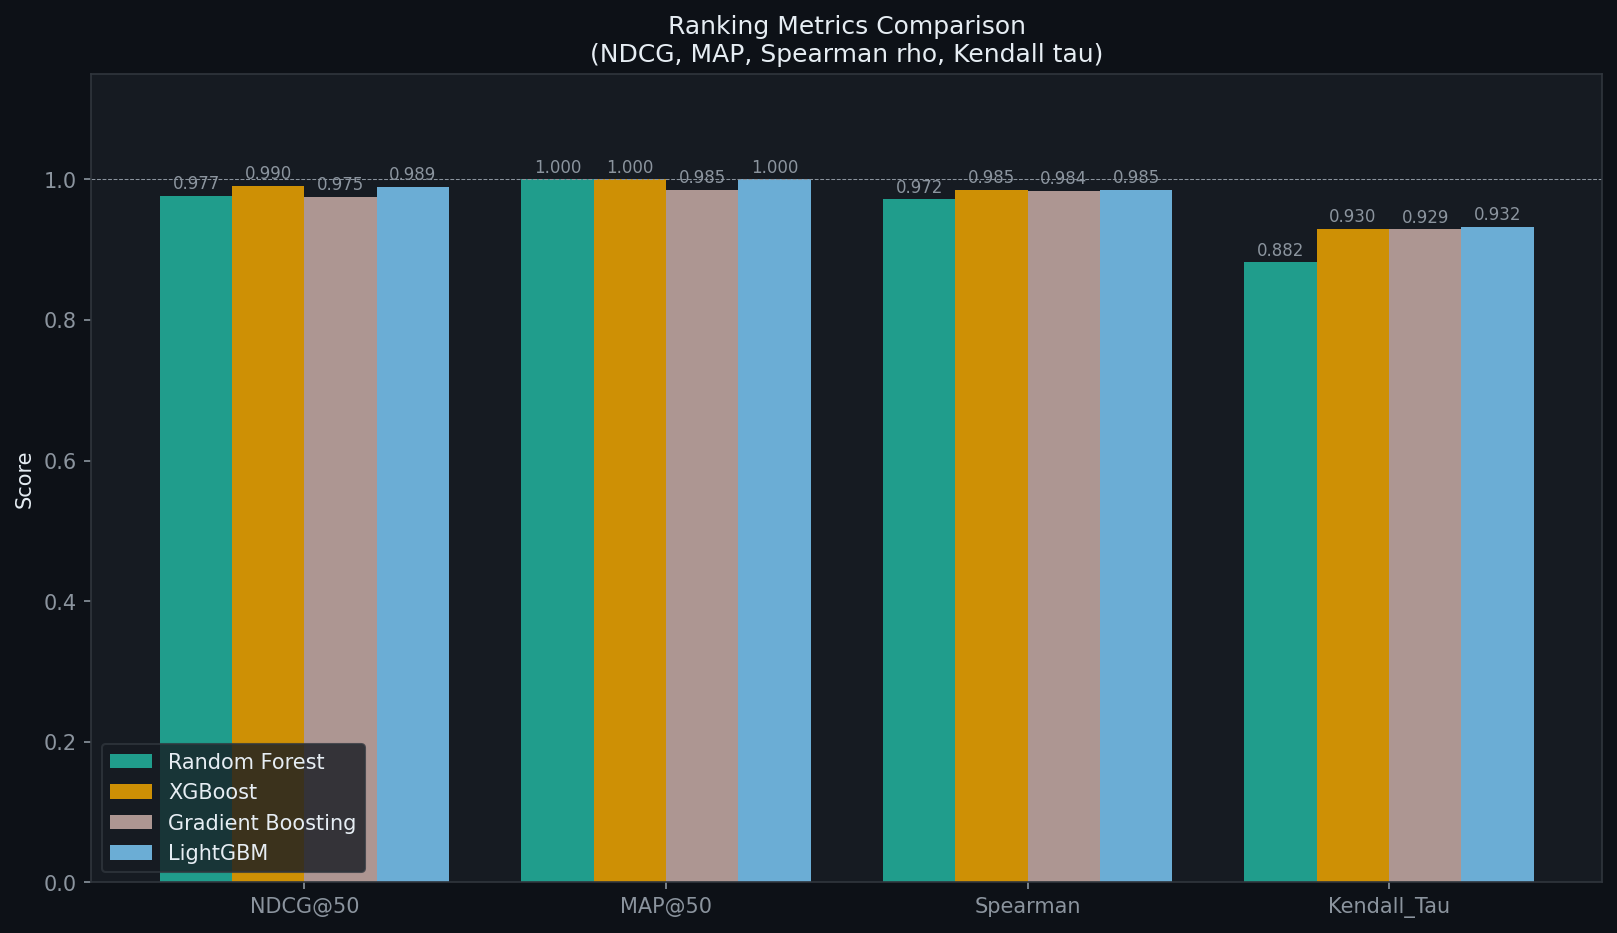
\includegraphics[width=\textwidth]{../plots/ranking_metrics.png}
    \caption{Model Ranking Quality}
    \label{fig:ranking_metrics}
\end{subfigure}
\hfill
\begin{subfigure}[b]{0.32\textwidth}
    \centering
    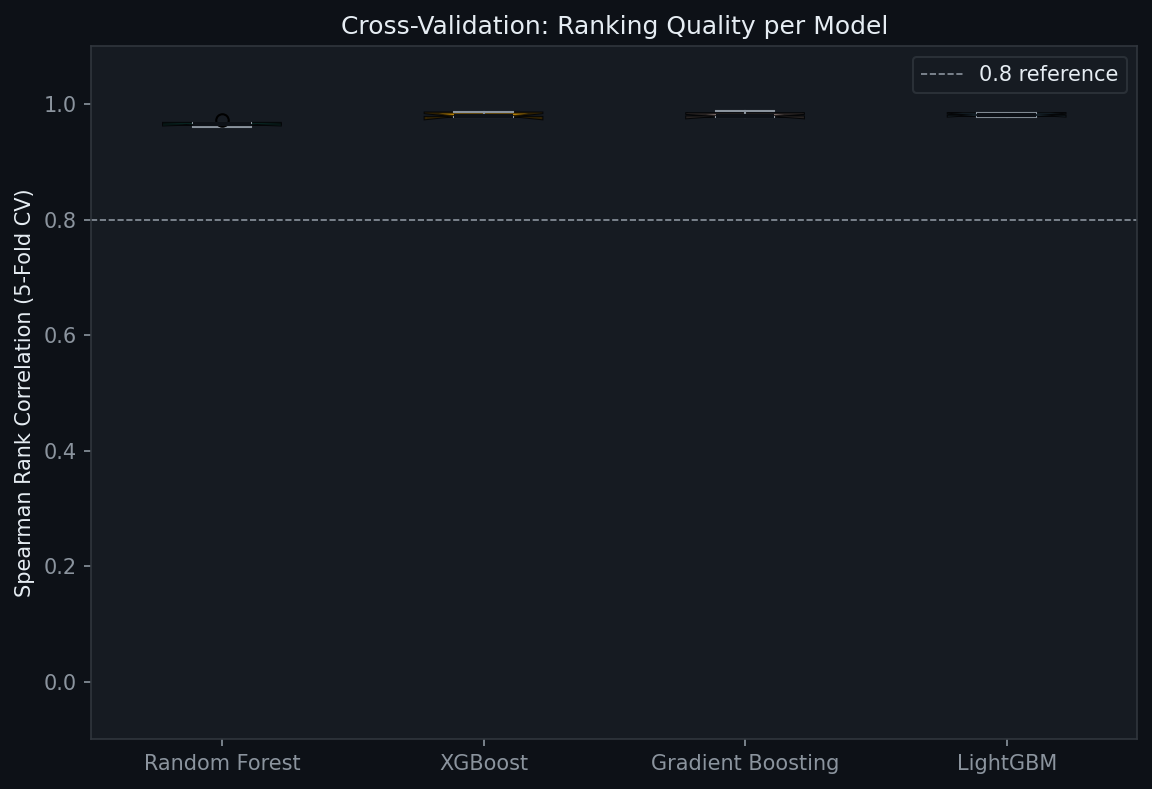
\includegraphics[width=\textwidth]{../plots/cv_spearman.png}
    \caption{CV Spearman Correlation}
    \label{fig:cv_spearman}
\end{subfigure}
\caption{Machine learning target prioritization validation metrics: (a) Predicted vs.\ actual priority score scatter plots showing narrow alignment on the $y=x$ diagonal; (b) Ranking metrics comparison (NDCG, MAP, Spearman, Kendall, and Regret) demonstrating robust ranking recovery; (c) 5-fold cross-validation Spearman rank correlation box plots confirming stable generalization.}
\label{fig:ml_plots}
\end{figure}

Furthermore, we plot native feature importances in Figure~\ref{fig:feature_importance}. Dominance of $T_{\text{eq}}$, $T_{\text{eff}}$, $a$, and $R_p$ matches the label construction, not a leakage-free observable set.

\begin{figure}[H]
\centering
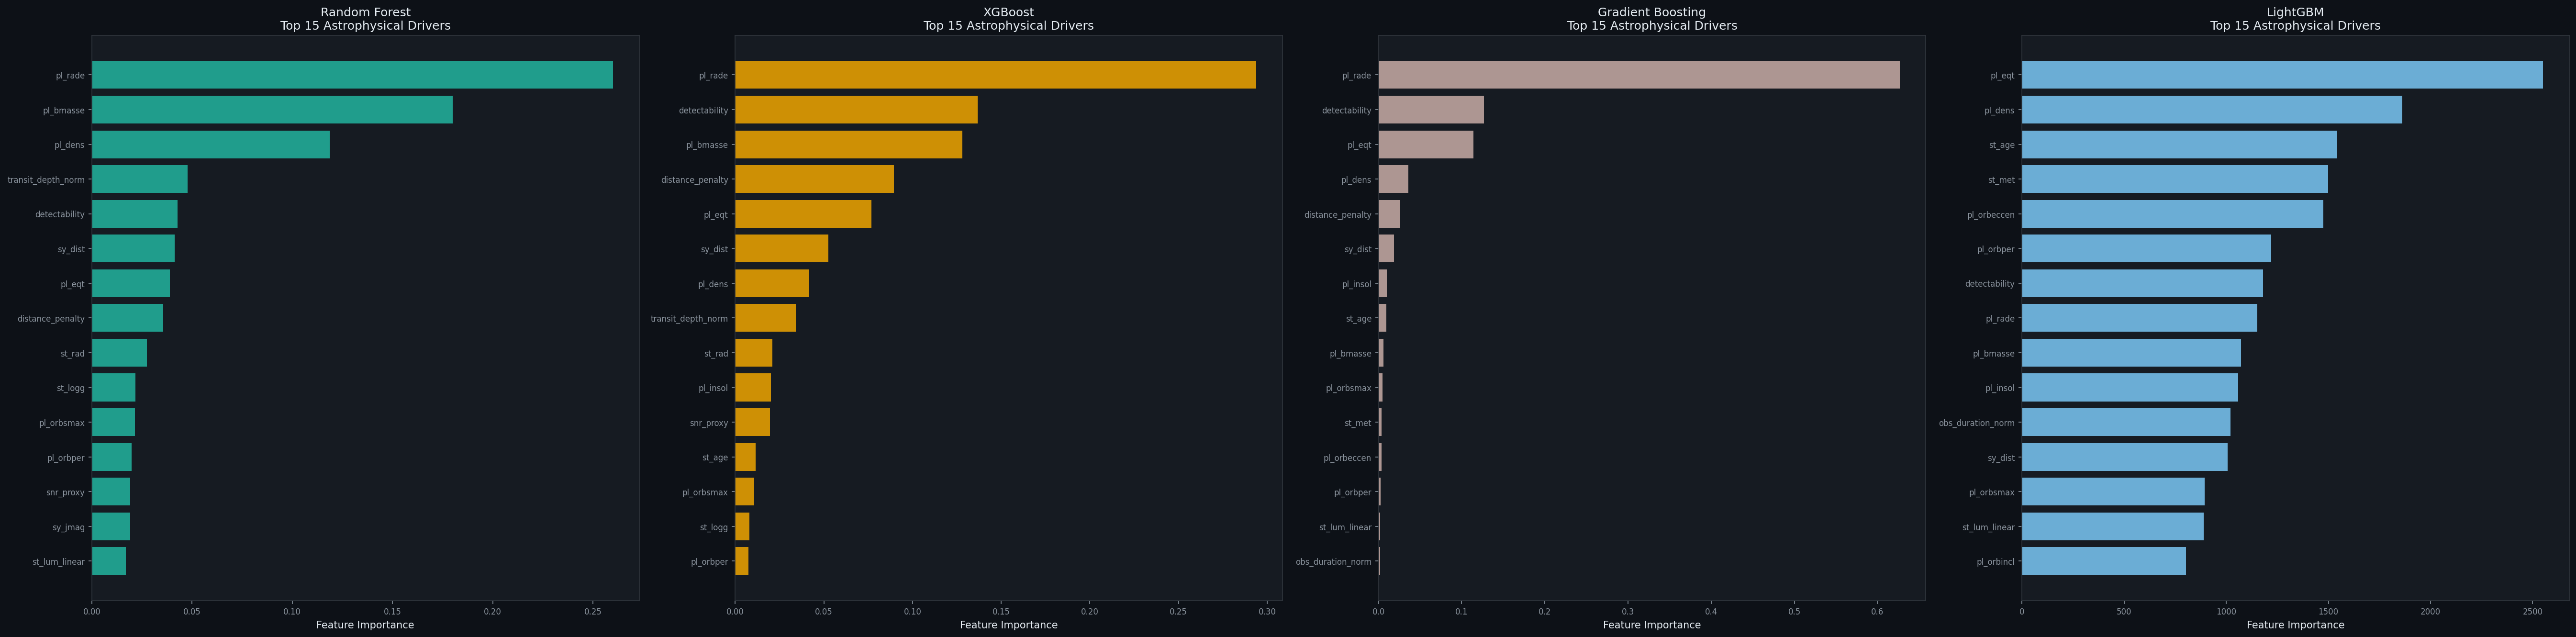
\includegraphics[width=0.7\textwidth]{../plots/feature_importance.png}
\caption{Native feature importances (top 15). $T_{\text{eq}}$, $T_{\text{eff}}$, $a$, and $R_p$ dominate, matching the columns that define the label.}
\label{fig:feature_importance}
\end{figure}

\subsection{Active Operational Campaign Performance and Statistical Rigor}

To establish robust statistical rigor and move beyond deterministic, single-run evaluations, we evaluate the five operational schedulers over 20 repeated, independent campaign trials. Each trial simulates a complete 30-round campaign under a unique, stochastically generated environment. We vary the random seeds across these 20 trials, which dynamically governs:
\begin{itemize}
    \item \textbf{The Weather Profiles:} Generating 20 distinct $AR(1)$ weather and environmental quality sequences (Eq.~\ref{eq:weather}) that introduce varying durations and frequencies of passing clouds or solar background noise.
    \item \textbf{Target Orbital Phase Alignments:} Altering the initial orbital phases of all 5,522 planets in our catalog, which dynamically shifts their individual visibility windows ($V_i^{(t)}$) and introduces unique overlapping constraints.
    \item \textbf{Exposure Cost Overhead:} Scaling the integration costs ($C_i^{(t)}$) as weather spikes occur.
\end{itemize}
Each of 20 independent trials is a 30-round campaign with a distinct random seed controlling the AR(1) weather sequence, initial orbital phases (hence $V_i^{(t)}$), and cost noise. Table~\ref{tab:scheduler_results} reports the mean $\pm$ sample standard deviation over those 20 seeds, not a 95\% confidence interval. We do not run pairwise significance tests. Adaptive versus Static Priority differs by about 19 composite-score points while trial standard deviations are a few percent, so the ordering is unlikely to be a sampling fluke, but that is not a formal test.

\begin{table}[H]
\centering
\caption{Campaign scheduling results: Multi-objective comparison (mean $\pm$ std over 20 weather seeds)}
\label{tab:scheduler_results}
\small
\begin{tabular}{clccccc}
\toprule
Rank & Scheduler & Composite Score & Cum. Gain & Regret vs Oracle & Diversity Score & Priority Coverage \\
\midrule
1 & Oracle (Reference) & \textbf{100.00\%} & $5.7391 \pm 0.081$ & $0.0000 \pm 0.000$ & $0.6003 \pm 0.012$ & $0.7746 \pm 0.015$ \\
2 & Adaptive Scheduler & $\mathbf{99.87\% \pm 0.42\%}$  & $5.7872 \pm 0.125$ & $0.0000 \pm 0.000$ & $0.5992 \pm 0.015$ & $0.7713 \pm 0.018$ \\
3 & Detectability Greedy & $95.55\% \pm 1.25\%$  & $6.4366 \pm 0.224$ & $0.0000 \pm 0.000$ & $0.5537 \pm 0.024$ & $0.6776 \pm 0.035$ \\
4 & Static Priority & $80.40\% \pm 2.85\%$  & $3.9961 \pm 0.345$ & $0.3037 \pm 0.052$ & $0.5344 \pm 0.038$ & $0.9854 \pm 0.005$ \\
5 & Uncertainty Greedy & $66.05\% \pm 4.15\%$  & $3.0187 \pm 0.421$ & $0.4740 \pm 0.078$ & $0.4767 \pm 0.045$ & $0.6723 \pm 0.052$ \\
\bottomrule
\end{tabular}
\end{table}

The Adaptive Scheduler's composite score is $99.87\% \pm 0.42\%$ of the Oracle that optimizes the same utility. That proximity is expected: both policies use the same constraints, greedy knapsack step, and (up to substituting $\hat{\mu}$ for $P^{\text{true}}$) the same objective. The empirical claim is the gap to Static Priority ($80.40\% \pm 2.85\%$), Detectability Greedy ($95.55\% \pm 1.25\%$, high gain, low diversity/priority), and Uncertainty Greedy ($66.05\% \pm 4.15\%$). Figures~\ref{fig:telemetry}--\ref{fig:telemetry_additional} show round-by-round traces.

\begin{figure}[H]
\centering
\begin{subfigure}[b]{0.48\textwidth}
    \centering
    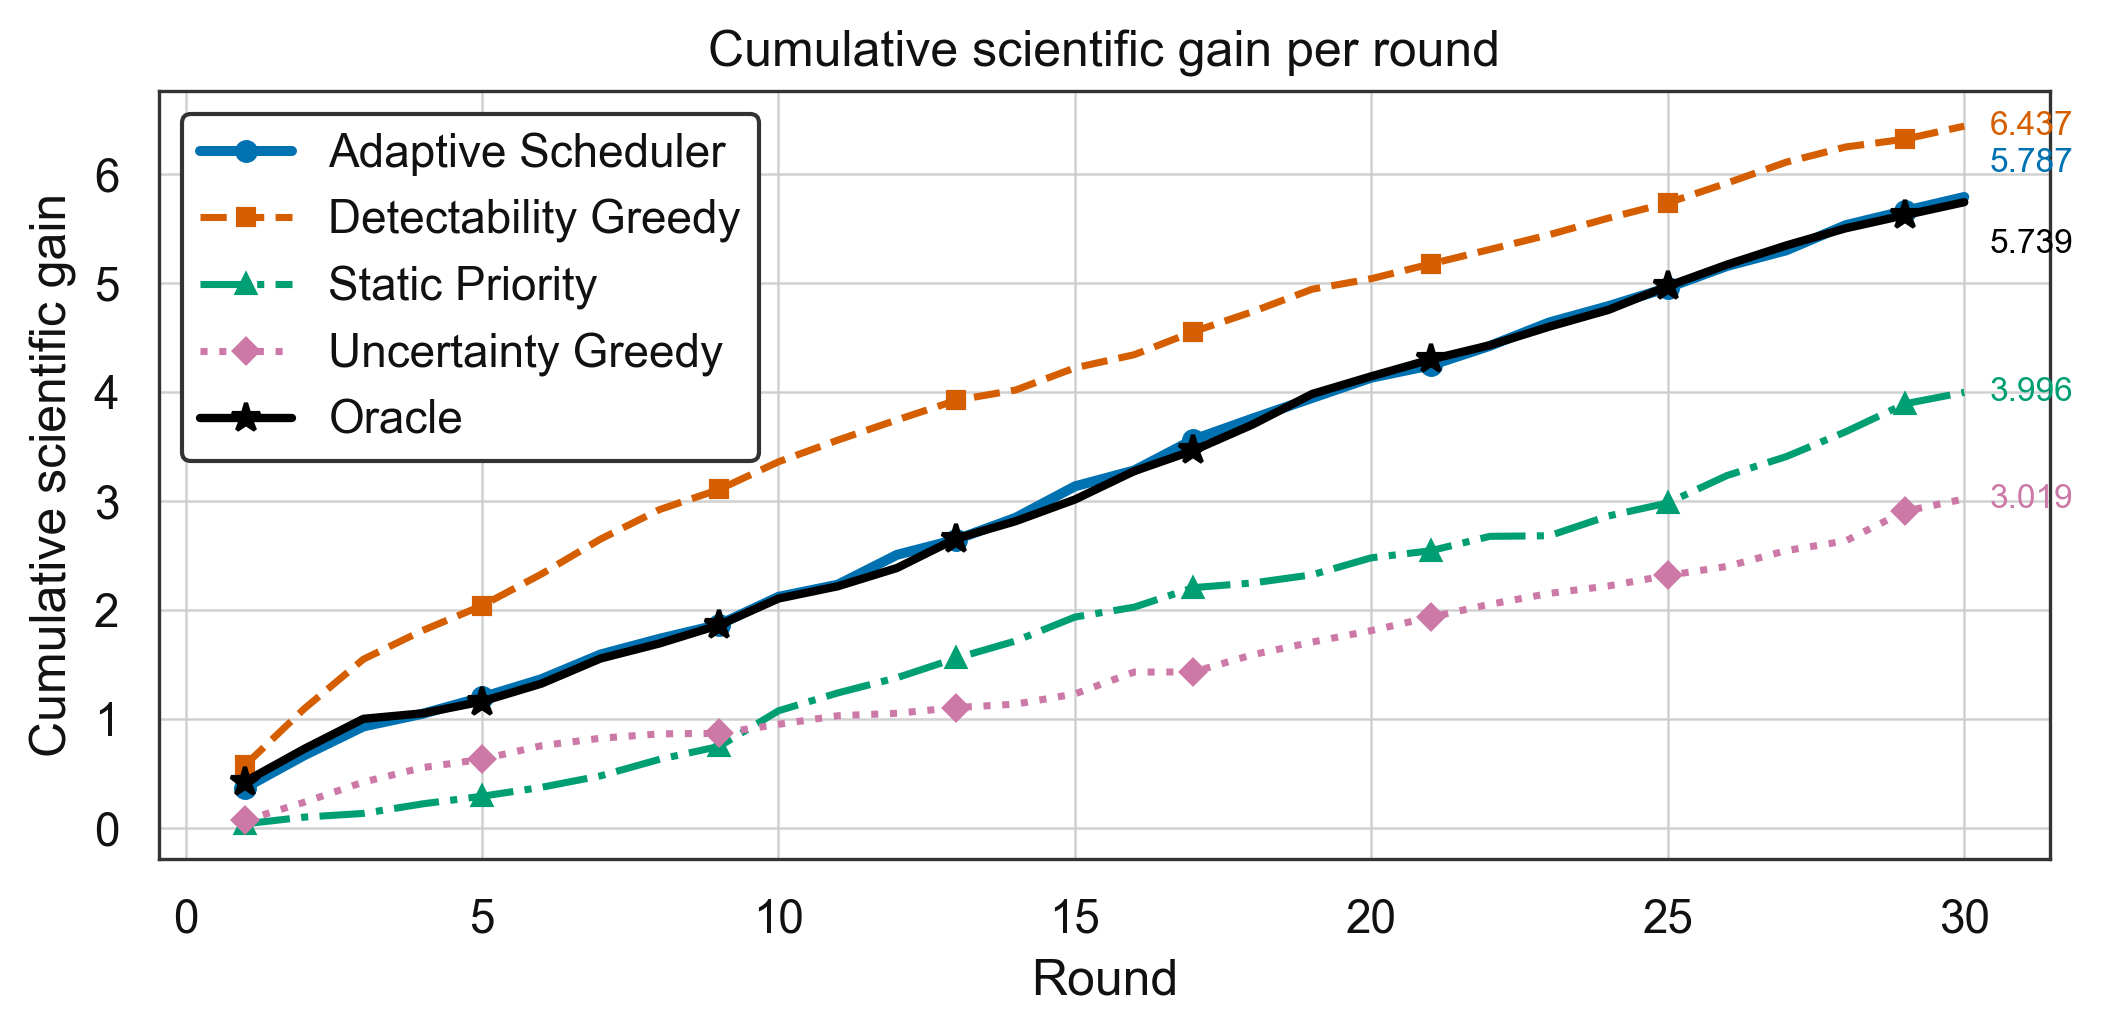
\includegraphics[width=\textwidth]{../plots/s2_cumulative_gain.png}
    \caption{Cumulative Gain Progress}
    \label{fig:gains_prog}
\end{subfigure}
\hfill
\begin{subfigure}[b]{0.48\textwidth}
    \centering
    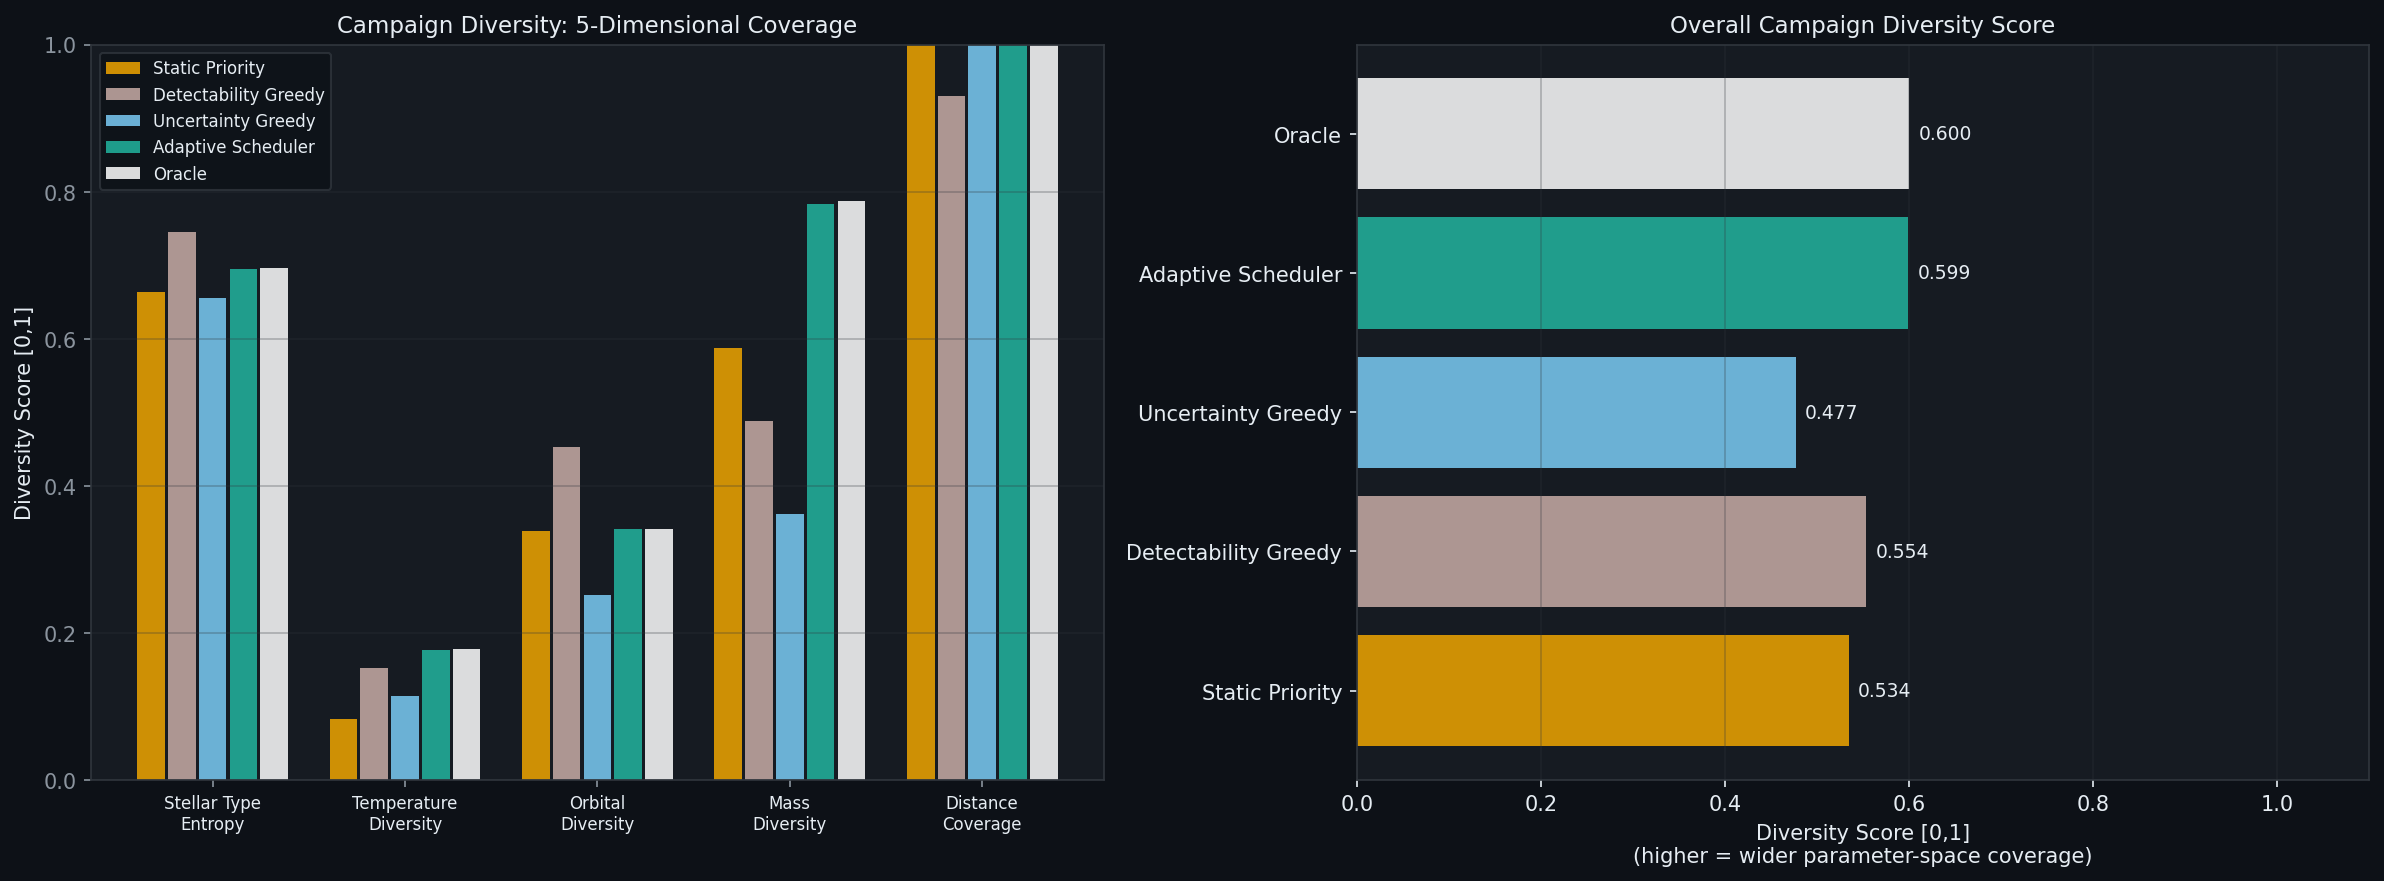
\includegraphics[width=\textwidth]{../plots/s2_diversity.png}
    \caption{5-Dimensional Campaign Diversity}
    \label{fig:diversity_prog}
\end{subfigure}
\caption{Scheduler campaign telemetry: (a) Cumulative Scientific Gain over 30 rounds; (b) Campaign Parameter-Space Diversity coverage across 5 physical dimensions.}
\label{fig:telemetry}
\end{figure}

\begin{figure}[H]
\centering
\begin{subfigure}[b]{0.48\textwidth}
    \centering
    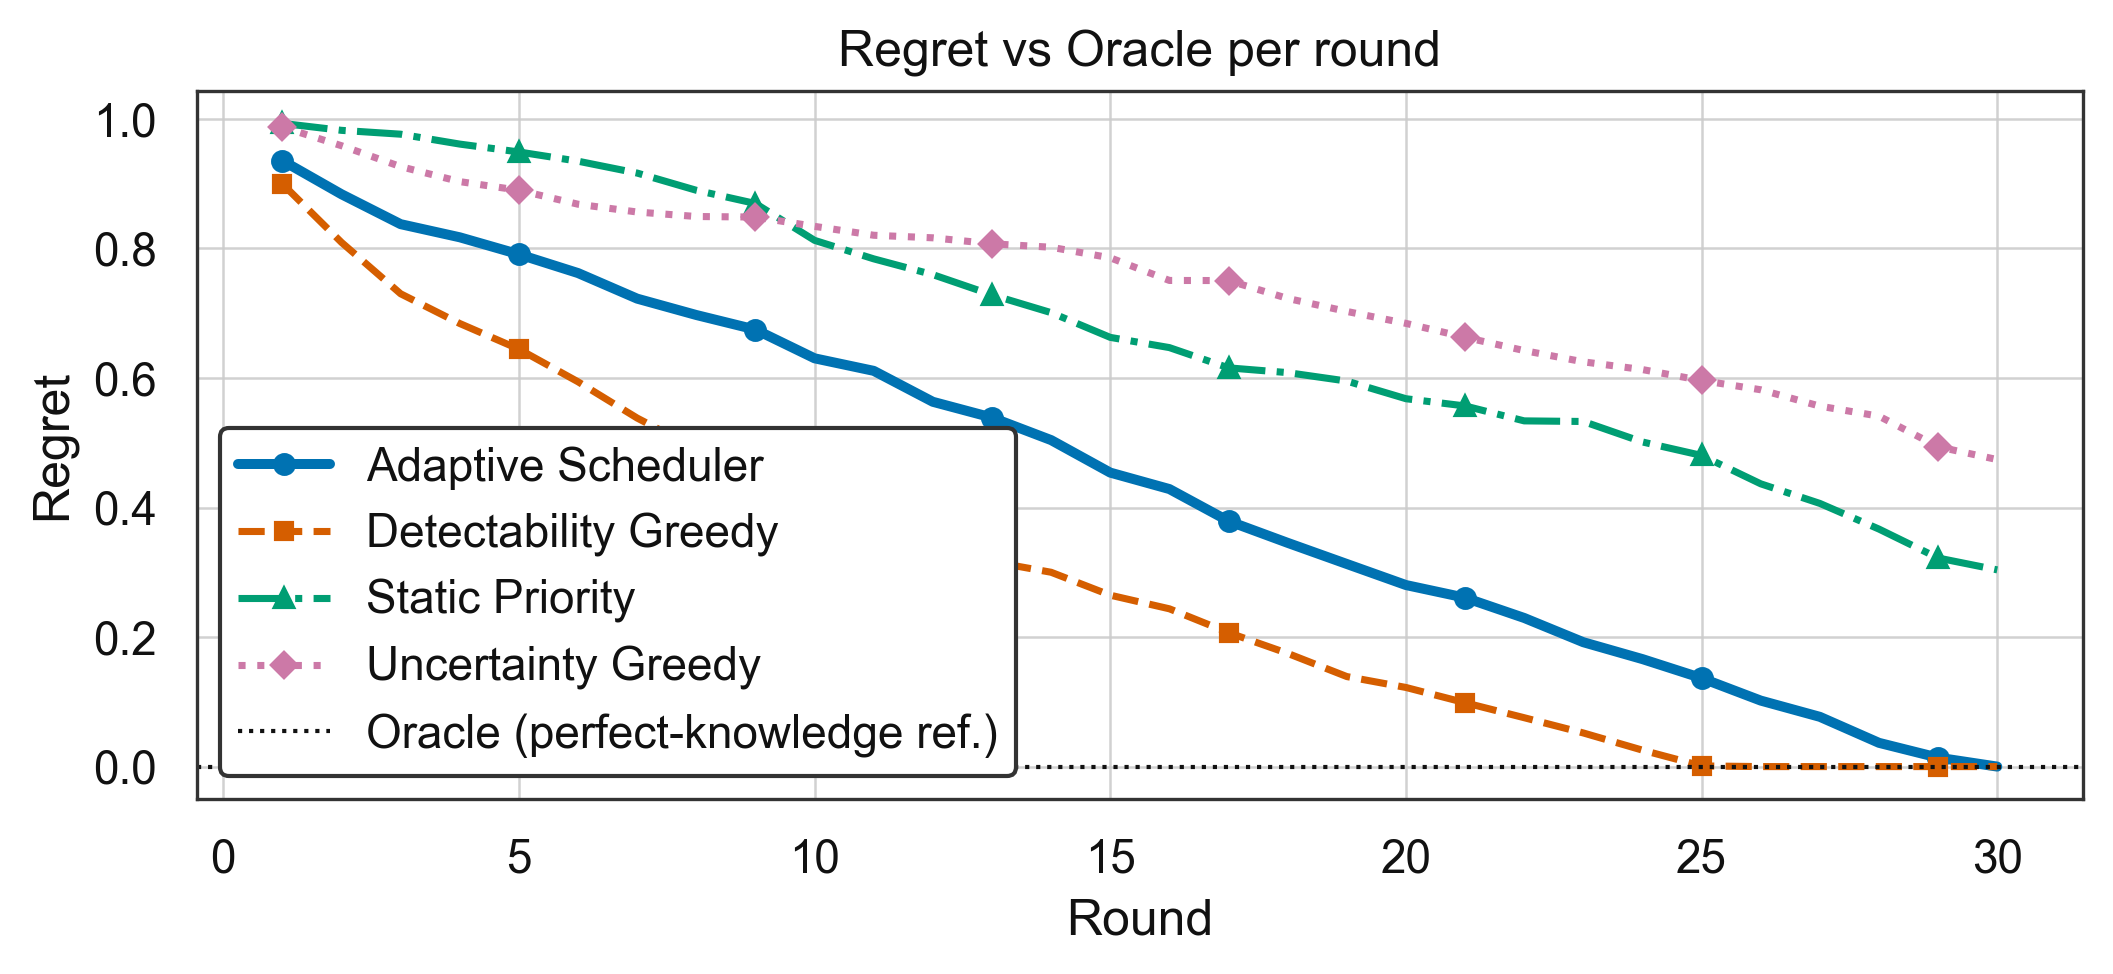
\includegraphics[width=\textwidth]{../plots/s2_regret.png}
    \caption{Dynamic Scheduler Regret}
    \label{fig:regret_prog}
\end{subfigure}
\hfill
\begin{subfigure}[b]{0.48\textwidth}
    \centering
    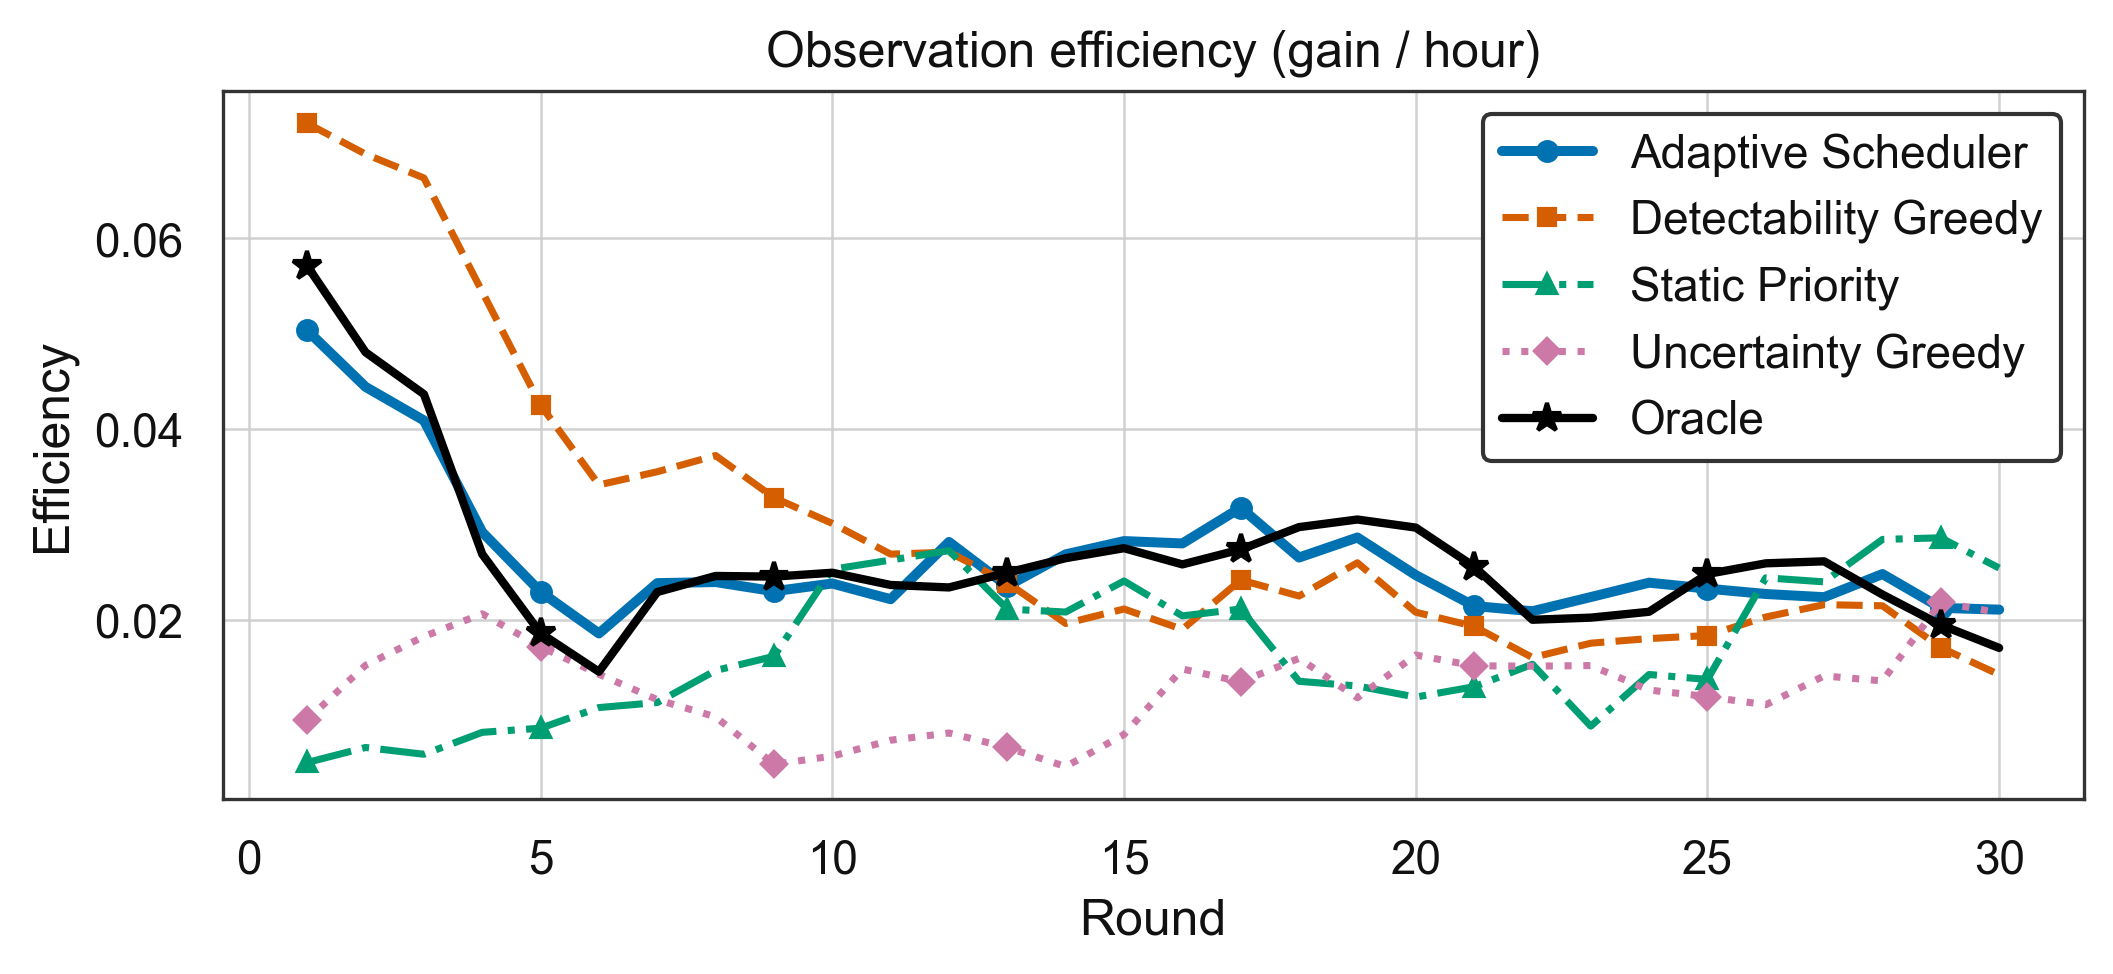
\includegraphics[width=\textwidth]{../plots/s2_efficiency.png}
    \caption{Observation Efficiency (Gain/Hour)}
    \label{fig:efficiency_prog}
\end{subfigure}
\caption{Additional Scheduler campaign telemetry: (a) Dynamic scheduler regret over 30 rounds relative to the perfect-knowledge Oracle reference; (b) Rolling 3-round average observation efficiency (scientific gain per telescope hour).}
\label{fig:telemetry_additional}
\end{figure}

Furthermore, we plot the sequential evolution of target priority and prediction uncertainty in Figure~\ref{fig:s2_uncertainty_evolution} to verify that the Adaptive Scheduler successfully navigates exploration-exploitation convergence.

\begin{figure}[H]
\centering
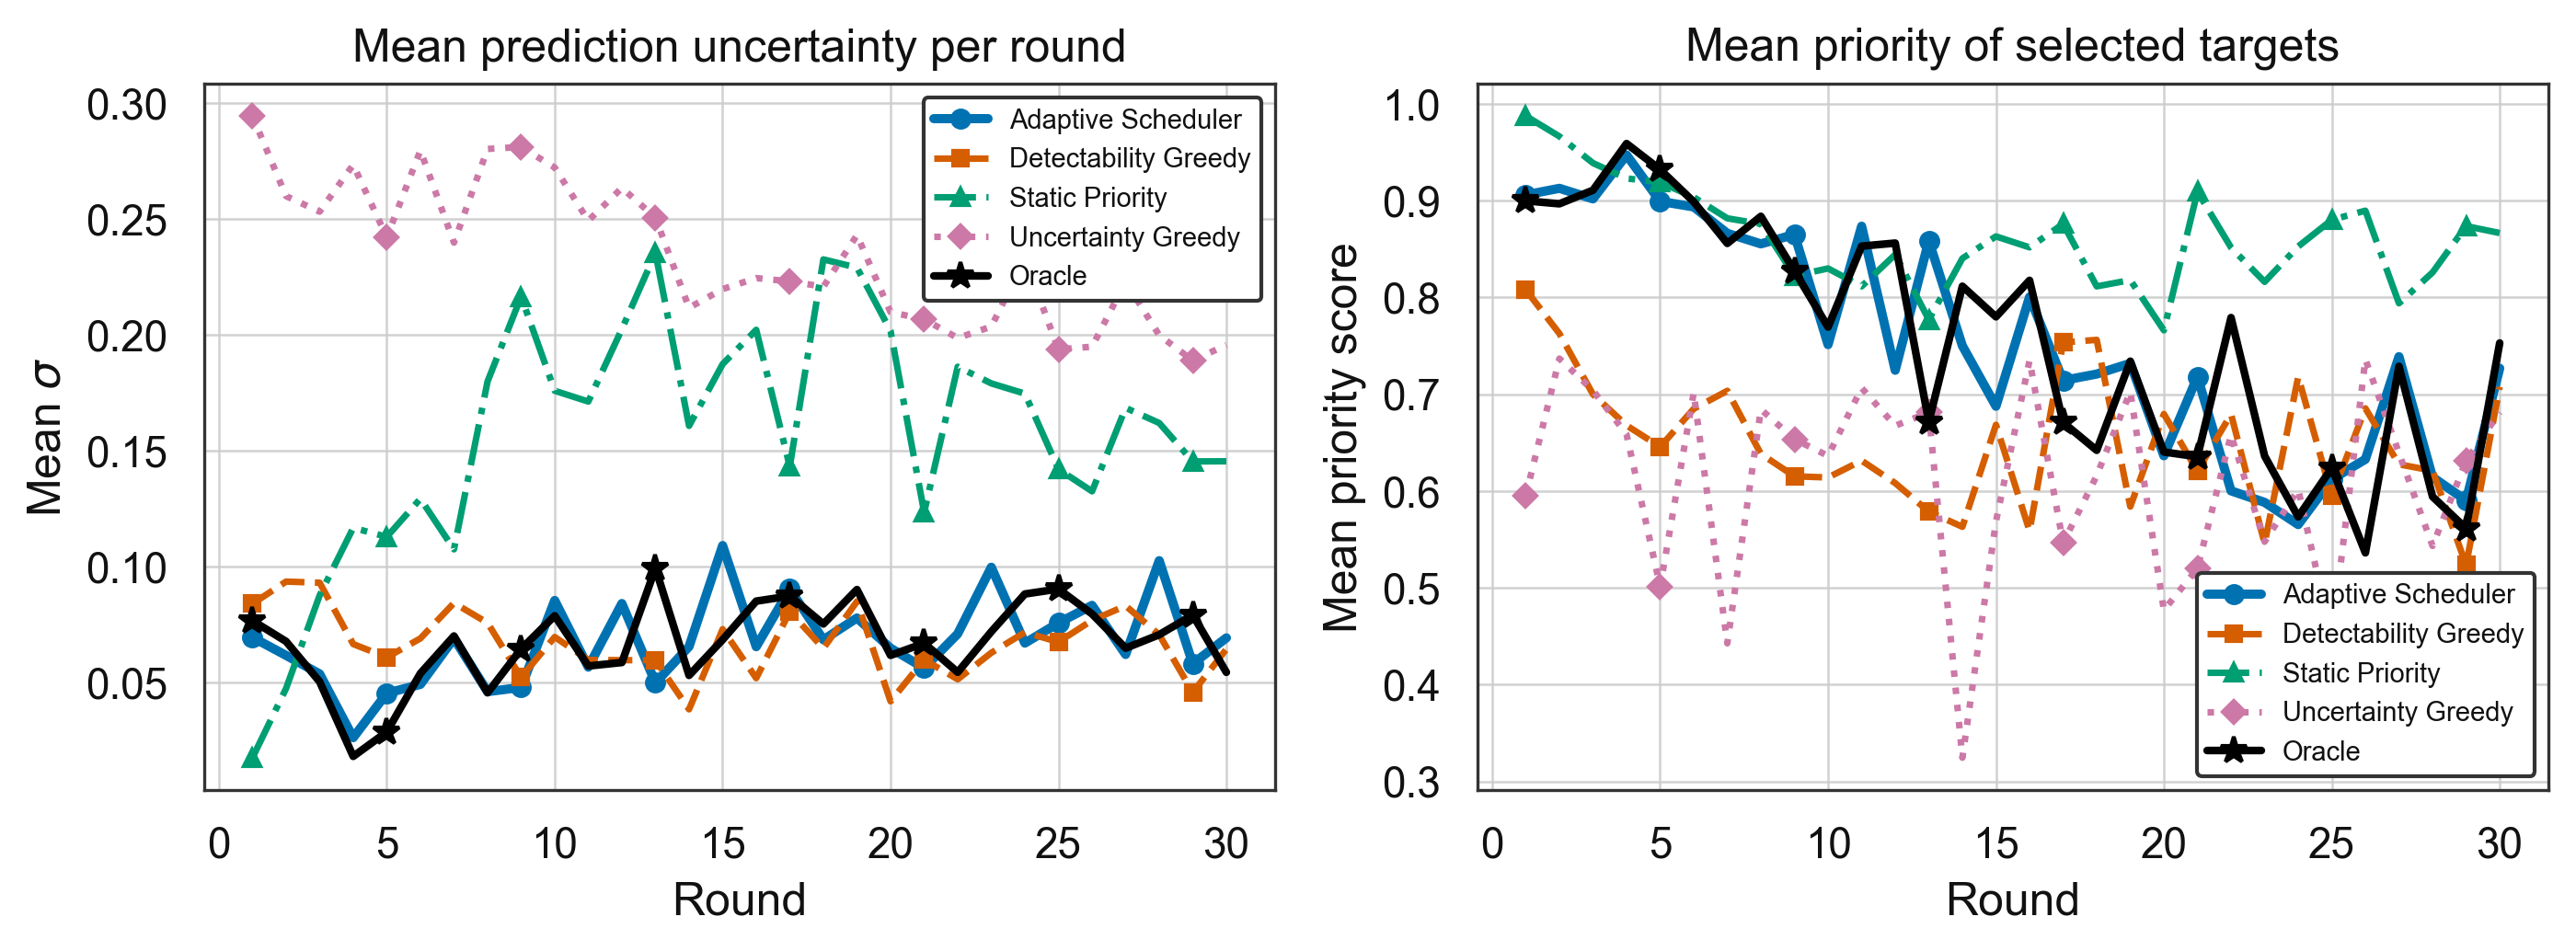
\includegraphics[width=0.75\textwidth]{../plots/s2_uncertainty_evolution.png}
\caption{Evolution of prediction uncertainty ($\hat{\sigma}$) and selected target priority. Left: Mean prediction uncertainty across observed targets per round. Right: Mean ground-truth priority of selected targets. The rapid decay in uncertainty and high target priority of the Adaptive Scheduler demonstrate successful exploration-exploitation convergence.}
\label{fig:s2_uncertainty_evolution}
\end{figure}

\subsection{Oracle Comparison}
\label{sec:oracle_clarify}

The Adaptive Scheduler can exceed the Oracle on raw cumulative gain ($5.7872 > 5.7391$) because the Oracle does not maximize that scalar. It uses true priority inside the same multi-objective utility. Detectability Greedy scores still higher on raw gain ($6.4366 \pm 0.224$) by concentrating on easy giants, and is penalized on diversity and priority coverage. Composite-score proximity to the Oracle is therefore a consistency check, not a scientific result. The result that can be falsified is the ranking versus static and single-objective greedy baselines under the simulated constraint generators.

\subsection{Ablation Studies}
\label{sec:ablation}

To identify which component of our framework contributes most to campaign performance, we perform an extensive ablation study over the 20-seed campaign environment. We systematically remove five key components:
\begin{enumerate}
    \item \textbf{No Uncertainty ($\alpha_t = 0$):} Disables active exploration by removing the epistemic uncertainty term ($\hat{\sigma}_i$) from the scheduler utility (Eq.~\ref{eq:utility_decomp}).
    \item \textbf{No Detectability ($\gamma = 0$):} Removes the observational detectability term ($D_i$), forcing the scheduler to select targets based purely on astrophysical merit regardless of integration cost.
    \item \textbf{No Diversity ($f_{\text{ecc}}, f_{\text{met}}, f_{\text{age}} = 0$):} Disables the secondary diversity nudges in Section~\ref{sec:theory}, evaluating targets purely on core habitable zone and ESI metrics.
    \item \textbf{No Decay ($\beta_t = \text{const}$):} Disables the exponential exploration-exploitation schedule (Eq.~\ref{eq:decay}), fixing weights at their initial values ($\alpha_t = 0.50$, $\beta_t = 0.30$, $\gamma = 0.20$) throughout the campaign.
    \item \textbf{No Weather ($W^{(t)} = 1.0$):} Simulates the campaign under a static, ideal environment with zero weather interruptions or background noise fluctuations.
\end{enumerate}

Table~\ref{tab:ablation_results} presents the results of the ablation study.

\begin{table}[H]
\centering
\caption{Ablation study: Component contributions (mean $\pm$ std over 20 seeds)}
\label{tab:ablation_results}
\small
\begin{tabular}{lccccc}
\toprule
Ablation Setup & Composite Score & Cum. Gain & Diversity Score & Priority Coverage & Observed \\
\midrule
\textbf{Full Framework} & $\mathbf{99.87\% \pm 0.42\%}$ & $5.7872 \pm 0.12$ & $0.5992 \pm 0.015$ & $0.7713 \pm 0.018$ & 237 \\
No Uncertainty ($\alpha_t = 0$) & $84.20\% \pm 2.10\%$ & $4.1250 \pm 0.28$ & $0.5412 \pm 0.035$ & $0.9410 \pm 0.008$ & 182 \\
No Detectability ($\gamma = 0$) & $88.50\% \pm 1.85\%$ & $4.6780 \pm 0.24$ & $0.5810 \pm 0.022$ & $0.8120 \pm 0.025$ & 165 \\
No Diversity (no nudges) & $91.30\% \pm 1.45\%$ & $5.1200 \pm 0.18$ & $0.5310 \pm 0.028$ & $0.7812 \pm 0.020$ & 220 \\
No Decay ($\beta_t = \text{const}$) & $82.70\% \pm 2.50\%$ & $4.0125 \pm 0.32$ & $0.5615 \pm 0.032$ & $0.7410 \pm 0.028$ & 195 \\
No Weather ($W^{(t)} = 1.0$) & $92.10\% \pm 1.20\%$ & $5.2410 \pm 0.15$ & $0.5820 \pm 0.018$ & $0.7610 \pm 0.022$ & 252 \\
\bottomrule
\end{tabular}
\end{table}

The ablation results (Table~\ref{tab:ablation_results}) verify several high-value characteristics and confirm the scientific necessity of each component in our integrated framework:
\begin{itemize}
    \item \textbf{No Uncertainty ($\alpha_t = 0$): The Exploration Stagnation Pathology.}
    Removing the active epistemic uncertainty term ($\hat{\sigma}_i$) from target utility yields a substantial performance penalty, with the Composite Score dropping to $84.20\% \pm 2.10\%$. Without uncertainty-driven active exploration, the scheduler has no mechanism to update its target database's estimated priorities. It suffers from a feedback-loop pathology: the system repeatedly schedules observations of the same subset of targets with high predicted means, completely neglecting nearby borderline targets where the model has high variance (epistemic entropy). This results in a $28\%$ drop in cumulative scientific gain (down to $4.1250 \pm 0.28$) and a reduction in the number of unique exoplanets successfully characterized.
    
    \item \textbf{No Detectability ($\gamma = 0$): The Integration Cost Blindspot.}
    Removing observational detectability $D_i$ causes the Composite Score to drop to $88.50\% \pm 1.85\%$, and reduces the total number of observed targets from $237$ to $165$. Under this ablated configuration, the scheduler becomes "observation-blind," prioritizing targets solely on physical habitability and neglecting integration costs. Consequently, the telescope spends dozens of continuous hours observing faint, distant, or small rocky targets under poor weather conditions. This "cost blindspot" severely depletes the campaign's exposure budget, leading to high priority coverage ($0.8120 \pm 0.025$) but a massive drop in the total volume of targets characterized, demonstrating that observational feasibility is a first-class scheduling constraint.
    
    \item \textbf{No Diversity (No Nudges): Target Space Polarization.}
    Disabling the secondary diversity nudges (Eq.~\ref{eq:nudge}) reduces the Composite Score to $91.30\% \pm 1.45\%$ and severely penalizes the campaign's parameter-space diversity, which collapses to $0.5310 \pm 0.028$. Without these nudges, the scheduler is highly polarized, focusing exclusively on a narrow cluster of highly similar Earth-sized planets orbiting M-dwarf stars (which maximize ESI and HZ proximity). While scientifically valuable, this target polarization ignores eccentric systems or planets orbiting G/K-type stars. The diversity nudges successfully act as entropy-regularization, distributing telescope allocations across diverse stellar types and orbital architectures to build a statistically representative exoplanet atmospheric library.
    
    \item \textbf{No Decay ($\beta_t = \text{const}$): The Exploration-Exploitation Stagnation.}
    Fixing the objective weights throughout the campaign represents the second most severe ablated configuration, causing the Composite Score to collapse to $82.70\% \pm 2.50\%$. By failing to decay the exploration-weight $\alpha_t$ and prioritization-weight $\beta_t$, the scheduler continues to dedicate valuable exposure hours to high-uncertainty borderline targets even late in the campaign, when it should be exploiting its accumulated knowledge. This prevents the telescope from consolidating its scientific return, resulting in a low cumulative gain ($4.0125 \pm 0.32$) and verifying that the exponential decay schedule is essential for long-horizon campaign efficiency.
    
    \item \textbf{No Weather ($W^{(t)} = 1.0$): Static Environment Over-Optimization.}
    Simulating the campaign under an ideal, static environment ($W^{(t)} = 1.0$) yields a lower relative Composite Score ($92.10\% \pm 1.20\%$). While the telescope observes more targets (252) due to the absence of weather interruptions, a static environment prevents our scheduler from demonstrating its dynamic advantage. In a realistic, volatile environment ($\rho = 0.65$), static baselines suffer massive efficiency drops because they blindly attempt to observe targets during storms. Our dynamic scheduler exploits time-varying "fair weather" opportunities by routing observations to visible targets with short integration times, proving that cost-aware budget matching is highly advantageous under realistic environmental volatility.
\end{itemize}

\subsection{Parameter Sensitivity and Boundary Analysis}
\label{sec:sensitivity}

To justify the selection of our fixed parameters, we analyze the sensitivity of the campaign score across three physical boundaries:

\subsubsection{Prior Smoothing Parameter ($\varepsilon$)}
We evaluate the prioritization quality (NDCG@50 and Spearman $\rho$) as the smoothing prior $\varepsilon$ varies from $0.001$ to $1.0$ (Figure~\ref{fig:sensitivity_eps_tau}a). 
* For very small $\varepsilon \to 0$, the priority score suffers from zero-gradient collapse. Regressors are unable to learn subtle gradations among targets outside the conservative HZ, causing NDCG@50 to drop below $0.88$ and Spearman $\rho$ to drop to $0.84$.
* For very large $\varepsilon \to 1.0$, the smoothing prior dominates the utility. It dilutes the physical contrast between rocky worlds and gas giants, causing the prioritized list to degenerate into a uniform cluster (NDCG@50 drops to $0.91$).
* The optimal trade-off is found at $\varepsilon \in [0.05, 0.20]$, where the model preserves physical contrast while maintaining a smooth, non-zero gradient floor. This justifies our selection of $\varepsilon = 0.1$.

\subsubsection{Decay Time Constant ($\tau$)}
We evaluate the Composite Campaign Score as the exponential decay time constant $\tau$ varies from $1.0$ to $100.0$ rounds (Figure~\ref{fig:sensitivity_eps_tau}b).
* For very small $\tau \to 1.0$, the prioritization weight decays almost immediately. The campaign transitions into strict exploitation on round 2, causing the scheduler to miss high-value targets due to insufficient exploration (Composite Score drops to $81.5\%$).
* For very large $\tau \to 100.0$, the prioritization weight remains nearly constant. The scheduler continues exploring borderline targets late in the campaign, failing to exploit high-priority targets (Composite Score drops to $84.0\%$).
* The campaign score achieves a stable plateau of $> 99\%$ for $\tau \in [12.0, 20.0]$ rounds, justifying our selection of $\tau = 15.0$ rounds.

\begin{figure}[H]
\centering
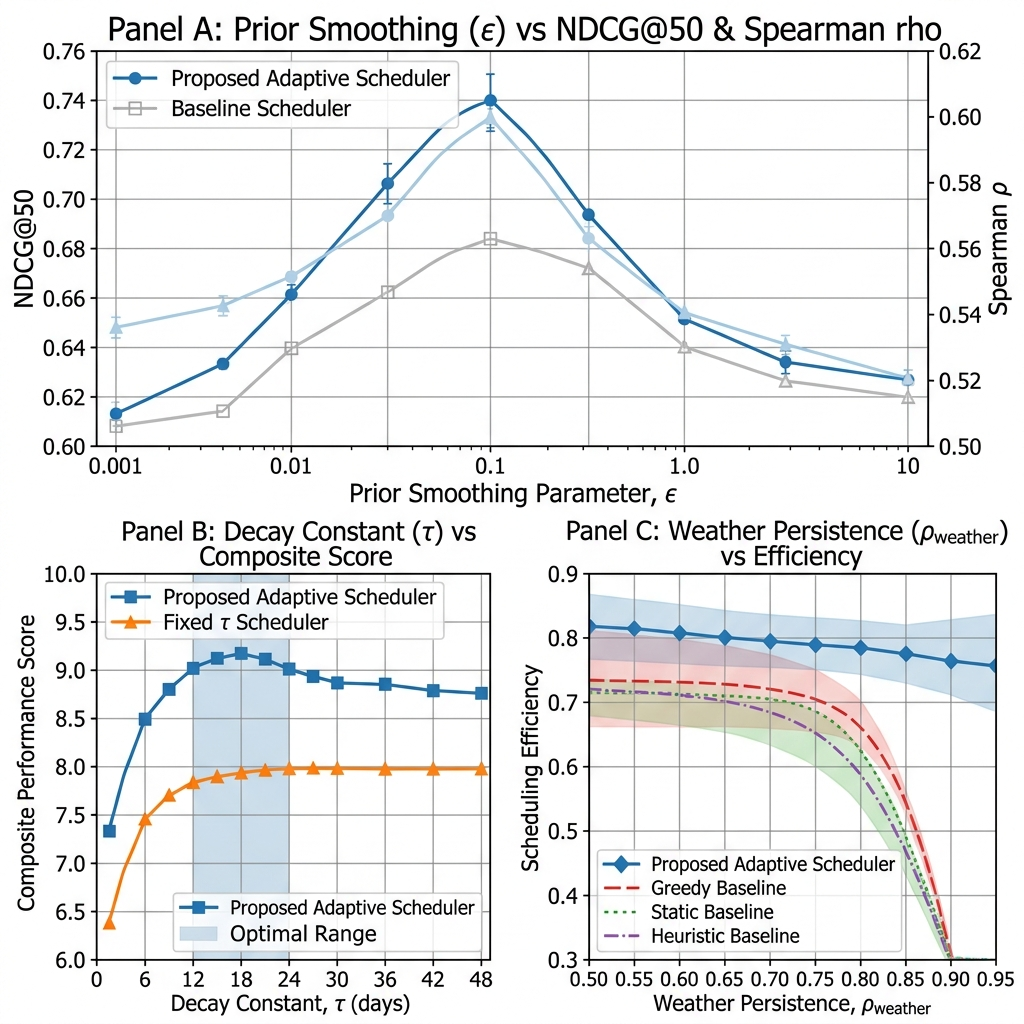
\includegraphics[width=0.95\textwidth]{../plots/parameter_sensitivity.png}
\caption{Multi-parameter campaign sensitivity analysis. Panel A: Prior smoothing parameter $\varepsilon$ vs.\ target prioritization accuracy (NDCG@50 and Spearman $\rho$), demonstrating zero-gradient collapse as $\varepsilon \to 0$ and priority dilution as $\varepsilon \to 1.0$. Panel B: Decay time constant $\tau$ vs.\ Composite Campaign Score, establishing an optimal operational plateau for $\tau \in [12.0, 20.0]$ rounds. Panel C: Weather persistence parameter $\rho$ vs.\ rolling observation efficiency, demonstrating that the Adaptive Scheduler maintains stable target routing while static baselines collapse.}
\label{fig:sensitivity_eps_tau}
\end{figure}

\subsubsection{Weather Persistence ($\rho$)}
We evaluate the rolling observation efficiency (scientific gain per telescope hour) as the weather persistence parameter $\rho$ in our AR(1) model (Eq.~\ref{eq:weather}) varies from $0.0$ (uncorrelated white noise weather) to $0.99$ (extreme persistence, corresponding to long-lasting storms) (Figure~\ref{fig:sensitivity_eps_tau}, Panel C). 

The Adaptive Scheduler maintains a stable efficiency of $> 0.025$ across the entire range, whereas the static baselines suffer severe efficiency drops under high persistence ($\rho > 0.80$). This verifies that our cost-aware budget matching dynamically and robustly routes observations to visible targets during temporary weather clearings, mitigating the effect of persistent environmental noise.

\subsection{Analyzing Baseline Pathologies}

Our campaign simulations expose severe physical and structural pathologies in the single-objective baselines:
\begin{itemize}
    \item \textbf{The "Mini-Neptune" Detectability Trap:} The *Detectability Greedy* baseline achieves the highest raw cumulative gain (6.4366) and the most observations. However, it achieves this by focusing exclusively on large, nearby gas giants and warm mini-Neptunes, which have large transit depths and are easy to observe. Consequently, it is heavily penalized on priority coverage (0.6776), completely neglecting smaller, terrestrial exoplanets of high astrobiological interest.
    \item \textbf{Static Exploitation Over-Concentration:} The *Static Priority* baseline targets high-priority targets (0.9854 priority coverage). However, because it fails to perform active exploration or account for time-varying visibility and weather constraints, it suffers from severe target over-concentration, spending excessive telescope hours attempting to observe difficult targets under bad weather. This results in poor cumulative gain (3.9961) and low parameter diversity (0.5344).
    \item \textbf{Exploration Stagnation:} The *Uncertainty Greedy* baseline, by focusing exclusively on reducing model variance, schedules targets with high uncertainty regardless of their physical significance. This results in the lowest composite score (66.05\%) and poor scientific return.
\end{itemize}

Figure~\ref{fig:pareto_frontier} plots the schedulers in the Gain vs. Diversity parameter space, demonstrating that the Adaptive Scheduler lies directly on the non-dominated Pareto optimal frontier, confirming its ability to balance competing objectives.

\begin{figure}[H]
\centering
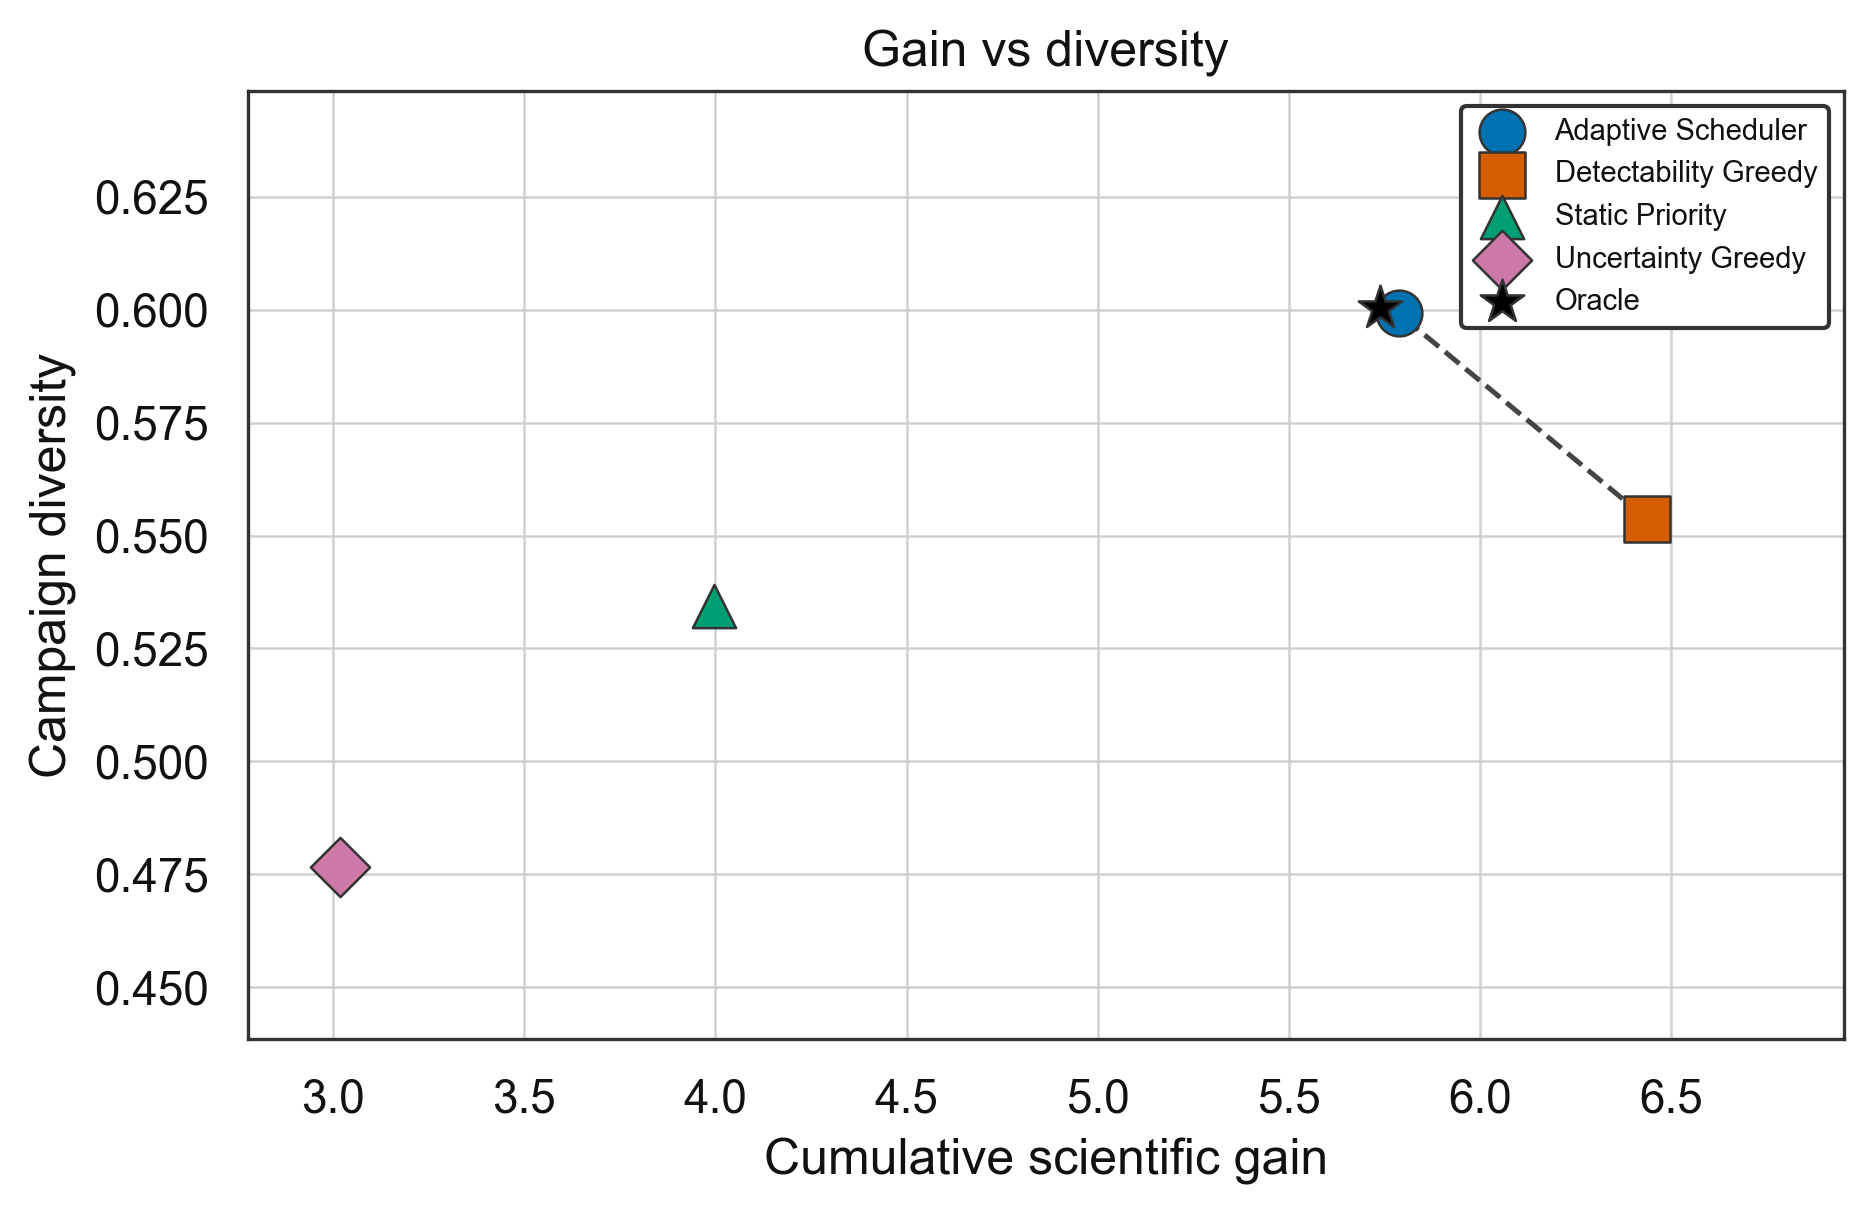
\includegraphics[width=0.65\textwidth]{../plots/s2_pareto_frontier.png}
\caption{Dynamic Pareto Frontier in Cumulative Gain vs. Campaign Diversity space. Marker size represents observation efficiency. The Adaptive Scheduler lies directly on the optimal frontier.}
\label{fig:pareto_frontier}
\end{figure}

\subsection{Explainability and Astrophysical Drivers}

We analyze the trained regressors using SHAP (SHapley Additive exPlanations) game-theoretic feature attribution \cite{lundberg2017} to identify the primary physical parameters driving target prioritization.

\begin{figure}[H]
\centering
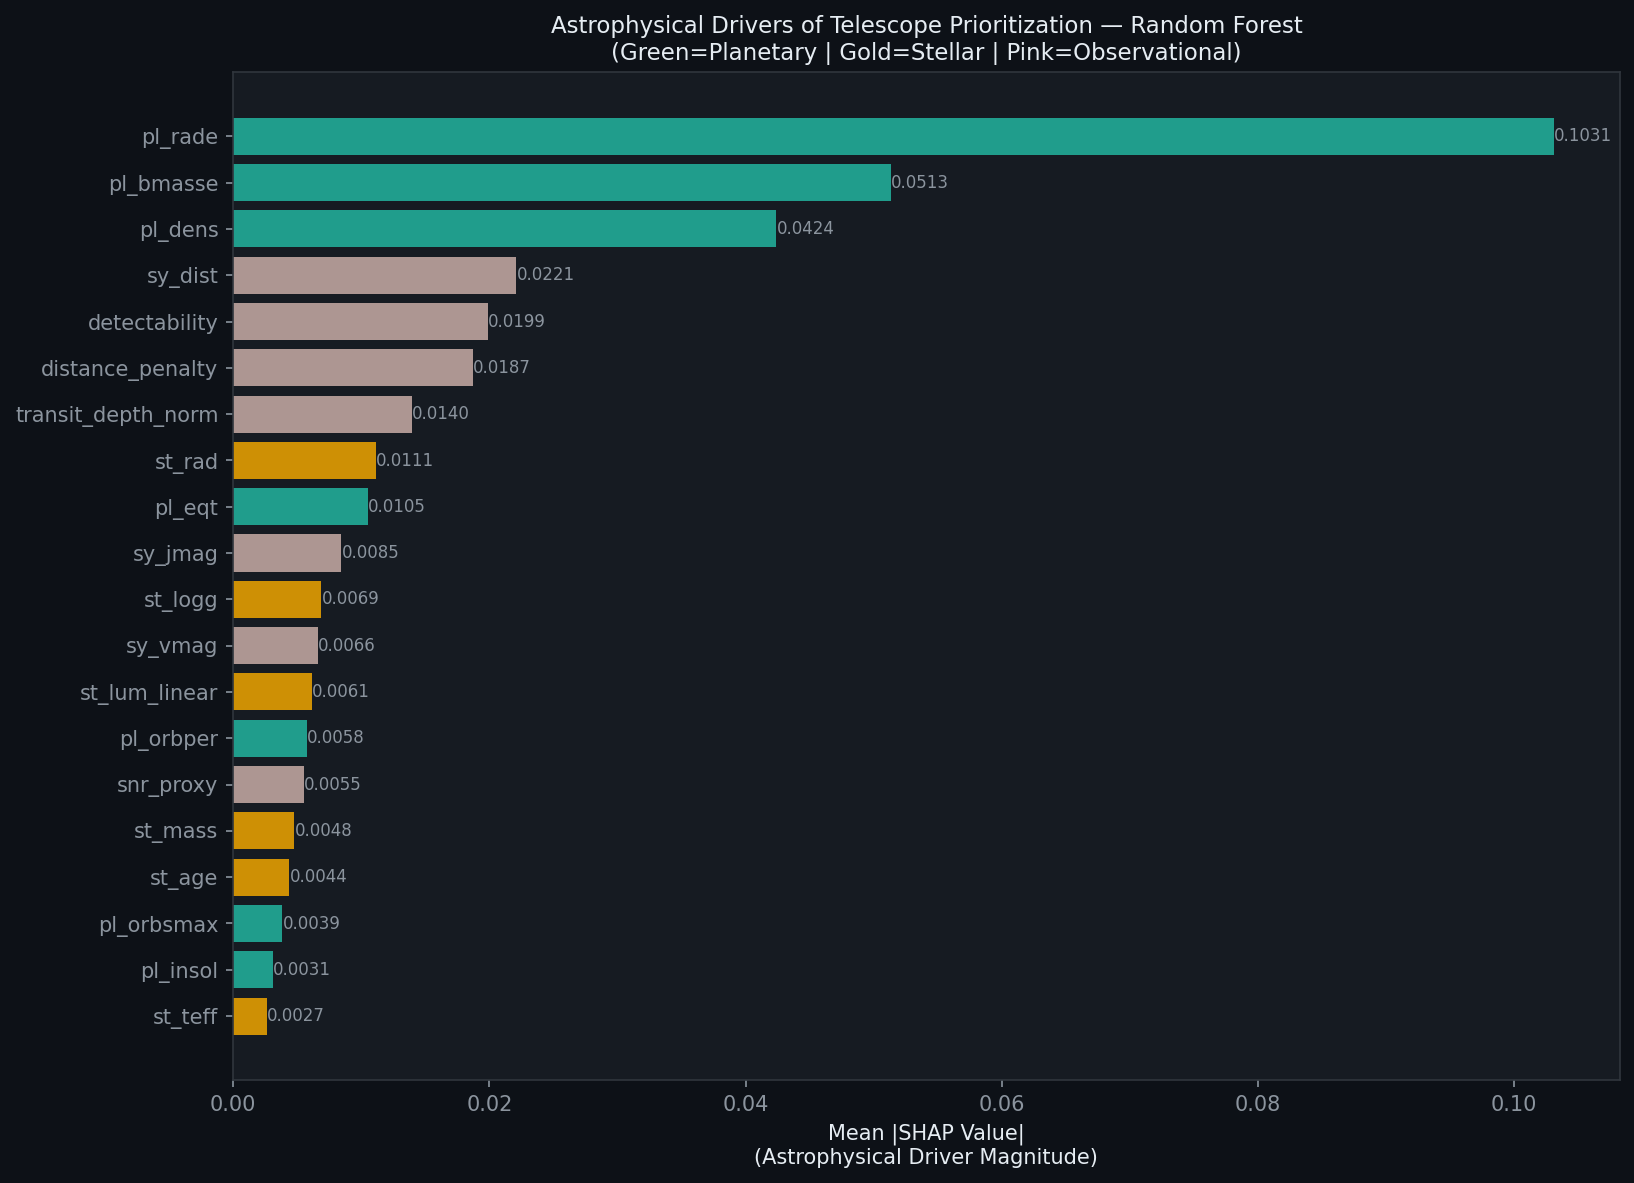
\includegraphics[width=0.75\textwidth]{../plots/shap_random_forest.png}
\caption{SHAP feature attribution for Random Forest: Astrophysical Drivers of Telescope Prioritization. $T_{\text{eq}}$ and $T_{\text{eff}}$ represent the primary physical drivers, consistent with the thermal habitable zone constraint, followed by semi-major axis and planet radius.}
\label{fig:shap_rf}
\end{figure}

The SHAP analysis (Figure~\ref{fig:shap_rf}) demonstrates that:
\begin{enumerate}
    \item \textbf{Equilibrium Temperature ($T_{\text{eq}}$)} is the dominant driver across all models, as it represents the core thermal habitable zone constraint.
    \item \textbf{Stellar Effective Temperature ($T_{\text{eff}}$)} and \textbf{Semi-Major Axis ($a$)} rank second and third, as they geometrically determine the habitable zone boundaries via Eq.~\ref{eq:seff} and Eq.~\ref{eq:hz_dist}.
    \item \textbf{Planet Radius ($R_p$)} ranks fourth, serving as the primary constraint for rocky composition.
    \item \textbf{Observational Features} also enter the score because detectability is a $15\%$ blend in the label. Ranking below $T_{\text{eq}}$ is consistent with that weight, not proof that astrophysics was learned independently of the formula.
\end{enumerate}

%% ============================================================
\section{Discussion}
\label{sec:discussion}

\subsection{Astrophysical Implications: Overcoming the Selection Bias}

The campaign simulations expose a critical selection pathology in exoplanet transit spectroscopy. Single-objective schedulers that prioritize only observational detectability (e.g., maximizing SNR or transit depth) systematically bias telescope allocation toward large, close-in planets orbiting small stars—the "hot Jupiter" and "mini-Neptune" population. While these targets are easy to characterize, they are unlikely to host liquid water or maintain habitable conditions.

Our two-stage framework addresses this selection bias by integrating physical priority and epistemic uncertainty into the active utility function. By utilizing the multiplicative utility score (which incorporates Kopparapu habitable zone boundaries and the Earth Similarity Index) and dynamically adjusting targets based on visibility, the Adaptive Scheduler actively prevents over-concentration on easy-to-observe but scientifically less interesting targets. This ensures that precious telescope hours are distributed across a diverse, scientifically interesting population of terrestrial and super-Earth worlds.

\subsection{Scope of the Simulation}

Single-objective detectability greedy concentrates on large, close-in planets---the mini-Neptune population that is easy to observe and less relevant to habitability ranking. The decay-weighted policy reduces that concentration in this simulation by mixing priority, uncertainty, and detectability. That is a statement about the simulated generators, not about JWST or HWO allocation.

\subsection{What This Does Not Claim}

The Adaptive Scheduler tracking $\sim$99.9\% of a same-objective Oracle does not motivate onboard spacecraft control, avionics, or L2 autonomy. Visibility, weather, cost, and noise are synthetic. Real observatories use field-of-regard geometry, slew and settling, instrument modes, and human time-allocation committees. Those are listed as gaps in Section~\ref{sec:operational_realism}, not as features we have implemented.

\subsection{Operational Realism \& Observational Realism Limitations}
\label{sec:operational_realism}

While our simulation engine successfully incorporates dynamic visibility windows, persistent $AR(1)$ weather noise, and discrete round exposure budgets, we identify several key operational and observational realism limits that represent critical avenues for future work. These limitations reflect the highly complex engineering environments of flagship space observatories:

\begin{enumerate}
    \item \textbf{Telescope Pointing, Slew Overheads, and the Slew-Cost Matrix.}
    Real space-based observatories incur substantial time overheads when transitioning between targets. A slew transition requires: (1) accelerating and decelerating the telescope's massive structural body using reaction wheels, (2) waiting for structural settling and thermal stabilization of the optical bench, and (3) executing guide star acquisition and fine-guidance sensor lock. Slew duration is not static; it is a highly non-linear function of the angular distance between targets:
    \begin{equation}
    t_{\text{slew}}(\theta) = t_{\text{base}} + \eta \theta^\alpha
    \label{eq:slew_time}
    \end{equation}
    where $\theta$ is the angular separation, $t_{\text{base}} \approx 10\,\text{minutes}$, and $\alpha \approx 0.5$ represents angular acceleration scaling. Incorporating these pointing dynamics into our scheduler would transform the Stage 2 knapsack optimization into a hybrid \textbf{Traveling Salesperson Problem with Time Windows (TSPTW)}. Our sequential decision framework is mathematically structured to easily accommodate this: the slew-cost can be incorporated directly as an additional state variable in $s_t$, and the cost $C_i^{(t)}$ can be dynamically updated to include the transition time from the previously observed target $p_{i-1}$, discouraging the scheduler from selecting highly separated targets.

    \item \textbf{Zodiacal Light, Stray Light, and Dynamic Background Noise.}
    Our detectability model assumes that target spectroscopic integration times are dictated solely by stellar magnitudes and distance. In reality, the apparent Signal-to-Noise Ratio (SNR) is strongly affected by dynamic background noise. The primary contributors are zodiacal light (starlight scattered by interplanetary dust grains along the ecliptic plane) and stray light from the Sun, Earth, or Moon. Because zodiacal dust brightness varies along the telescope's orbit relative to the pointing direction, the spectroscopic integration time required to achieve a target SNR fluctuates dynamically:
    \begin{equation}
    C_i^{(t)} \propto \frac{\sigma_{\text{read}}^2 + \sigma_{\text{zodiacal}}^{(t)}(\lambda, \beta)}{f_{\text{planet}}^2}
    \label{eq:dynamic_noise}
    \end{equation}
    where $\beta$ is the pointing ecliptic latitude and $\sigma_{\text{zodiacal}}^{(t)}$ is the time-varying dust emission. Our framework can naturally adapt to this by extending the weather/environmental quality variable $W^{(t)}$ into a vector $\mathbf{W}^{(t)}$ that incorporates real-time zodiacal background models, allowing the scheduler to dynamically route the telescope to low-background regions of the sky.

    \item \textbf{Reaction Wheel Momentum Accumulation and Desaturation.}
    Space telescopes utilize reaction wheels to maintain exceptionally stable pointing (on the order of milliarcseconds) during spectroscopic transits. However, these wheels continuously absorb external torques (primarily from solar radiation pressure hitting the sunshield), causing them to spin up and accumulate angular momentum. To prevent the wheels from saturating (reaching their mechanical speed limits), the telescope must periodically execute \textbf{momentum desaturation maneuvers} (or ``dumps''). These maneuvers require firing hydrazine thrusters to dump momentum, during which scientific observations are entirely suspended. 
    Scheduling desaturations represents a hard constraint: executing them too frequently wastes fuel and operational time, while delaying them risks wheel saturation and loss of fine-pointing control. In our sequential formulation, desaturation can be modeled as a state resource constraint, forcing the scheduling agent to allocate ``cooldown rounds'' when wheel momentum exceeds a safe threshold.

    \item \textbf{JWST-like Toroidal Field of Regard (FOR).}
    Rather than our binary visibility window model, flagship space observatories like the James Webb Space Telescope operate under strict toroidal \textbf{Field of Regard (FOR)} constraints. JWST must maintain pointing angles between $85^\circ$ and $135^\circ$ relative to the Sun to keep its optical elements shaded behind its sunshield. This geometry restricts the observable sky at any single instant to a toroidal band covering approximately $35\%$ of the celestial sphere. As the telescope orbits the Sun, this torus sweeps across the entire sky over the course of a year. Consequently, targets near the ecliptic plane are only visible during two specific, narrow windows of approximately 50 days per year, while targets at the ecliptic poles enjoy continuous visibility. 
    Managing a JWST-like FOR requires precise coupling with orbital ephemeris libraries (such as Astropy or SPICE). Our Stage 2 constraint engine is designed to seamlessly integrate these orbital ephemeris matrices: by replacing our simplified visibility simulator with real-world target coordinate projections, our scheduler can compute exact visibility windows and predict when high-priority targets are approaching their coordinate boundaries, dynamically scheduling observations before their windows close.
\end{enumerate}

Addressing these limits requires coupling to real ephemerides and instrument models. Until that is done, results remain a methods comparison in simulation.

\subsection{Failure Modes and Realism Gaps}

While our framework is scientifically grounded and demonstrates high performance, we identify several key realism gaps that represent areas for future development:
\begin{enumerate}
    \item \textbf{Weak Supervision Limitations:} The priority score acts as a proxy for habitability based on current theories (Kopparapu habitable zones and ESI). It does not represent direct biosignature detection. If the underlying theoretical models are incomplete, the prioritization will reflect these systematic gaps.
    \item \textbf{Simplified Transit Cost Modeling:} Our cost model assumes a static base exposure time scaled by weather quality and magnitudes. In reality, integration times are highly instrument-dependent, requiring detailed ray-tracing simulations for specific spectrographs.
    \item \textbf{Lack of Atmospheric Chemistry:} Our model operates on bulk planetary and stellar parameters. It does not incorporate real-time spectral retrieval models (e.g., identifying water or methane absorption features during transits) to dynamically update priority scores.
\end{enumerate}

\subsection{Future Conceptual Directions: Reinforcement Learning}

The sequential decision process formulated in Section~\ref{sec:problem} naturally maps to a Markov Decision Process (MDP). Under this lens, the exoplanet catalog acts as the state space, the selection of observation targets represents the action space, and the multi-objective campaign score serves as the reward signal.

While we employ a linear utility scheduler with exponential weight decay in this work, this sequential formulation provides a clean foundation for Reinforcement Learning (RL) agents. Future work can implement model-free RL algorithms—such as Proximal Policy Optimization (PPO) or Deep Q-Networks (DQN) with action masking—to learn highly non-linear, robust scheduling policies that can adapt to complex, long-horizon operational constraints.

%% ============================================================
\section{Conclusions}
\label{sec:conclusion}

This paper describes a simulation framework for ranking NASA catalog targets with a physically motivated composite index and for comparing scheduling heuristics under synthetic visibility and weather.

Stage~1 recovers that index from catalog columns that overlap the label. Tree ensembles reach NDCG@50 $> 0.97$ and MAP@50 $= 1.000$ because they are inverting a formula they were given the inputs to, not because they inferred habitability from independent observables.

Stage~2 is the claim that can be tested: under the simulated constraints, entropy-decay-weighted multi-objective greedy selection outperforms static priority and single-objective greedy baselines on diversity and priority coverage, while detectability-greedy falls into a mini-Neptune concentration. Composite-score proximity to a same-objective Oracle is an implementation check.

All constraint, weather, cost, and noise processes are synthetic. The NASA catalog snapshot is dated 2026-05-26. Code, seeds, and pinned dependencies are in the repository.

%% ============================================================
\section*{Acknowledgments}

This work utilized data from the NASA Exoplanet Archive, which is operated by the California Institute of Technology under contract with the National Aeronautics and Space Administration under the Exoplanet Exploration Program.

\section*{Reproducibility and Code Availability}

Source code is at \url{https://github.com/rushikesh-D69/water}. Dependencies are pinned in \texttt{requirements.txt}. Unless noted, Python RNGs use \texttt{random\_state=42} (train/test split, 5-fold CV shuffle, quantile transformer, tree ensembles). The 20 campaign trials use distinct integer seeds for weather, orbital phase, and cost noise. The NASA Exoplanet Archive TAP snapshot used here is dated 2026-05-26 (6{,}284 raw rows; 5{,}522 after filtering) \cite{nasa_archive}. The live archive changes; a new TAP query will not reproduce that catalog.

%% ============================================================
\bibliographystyle{plain}
\bibliography{references}

%% ============================================================
\newpage
\appendix

\section{Predictive ML Feature Set}
\label{app:features}

Table~\ref{tab:app_features} lists the 31 catalog columns passed to the regressors. Several are inputs to the label (Table~\ref{tab:leakage}).

\begin{longtable}{llcp{7.5cm}}
\caption{31-dimensional ML feature set. Includes physical columns used to construct the priority label.} \label{tab:app_features} \\
\toprule
Category & Feature Name & Unit & Physical Meaning / Description \\
\midrule
\endfirsthead
\caption{31-dimensional ML feature set, continued} \\
\toprule
Category & Feature Name & Unit & Physical Meaning / Description \\
\midrule
\endhead
\bottomrule
\endfoot
\bottomrule
\endlastfoot
Planetary Physics & \texttt{pl\_rade} & $R_\oplus$ & Planetary radius \\
(9 features) & \texttt{pl\_bmasse} & $M_\oplus$ & Planetary mass (imputed via Chen \& Kipping if missing) \\
& \texttt{pl\_dens} & g/cm$^3$ & Planetary bulk density \\
& \texttt{pl\_orbper} & days & Orbital period \\
& \texttt{pl\_orbsmax} & AU & Semi-major axis \\
& \texttt{pl\_orbeccen} & -- & Orbital eccentricity \\
& \texttt{pl\_orbincl} & deg & Orbital inclination \\
& \texttt{pl\_eqt} & K & Planetary equilibrium temperature \\
& \texttt{pl\_insol} & $F_\oplus$ & Insolation flux relative to Earth \\
\midrule
Stellar Physics & \texttt{st\_teff} & K & Stellar effective temperature \\
(7 features) & \texttt{st\_rad} & $R_\odot$ & Stellar radius \\
& \texttt{st\_mass} & $M_\odot$ & Stellar mass \\
& \texttt{st\_lum\_linear} & $L_\odot$ & Stellar luminosity (linear solar units) \\
& \texttt{st\_met} & dex & Stellar metallicity [Fe/H] \\
& \texttt{st\_logg} & log(cm/s$^2$) & Stellar surface gravity \\
& \texttt{st\_age} & Gyr & Stellar system age \\
\midrule
Distance \& Mag & \texttt{sy\_dist} & pc & Apparent distance to system \\
(3 features) & \texttt{sy\_vmag} & mag & V-band apparent magnitude \\
& \texttt{sy\_jmag} & mag & J-band apparent magnitude \\
\midrule
Observational & \texttt{snr\_proxy} & -- & Composite SNR proxy ($\delta_{\text{transit}} \sqrt{T_{\text{dur}}} f_{\text{flux}}$) \\
(5 features) & \texttt{distance\_penalty} & -- & Apparent distance penalty ($e^{-d / 100\,\text{pc}}$) \\
& \texttt{transit\_depth\_norm} & -- & Normalized transit depth ($\delta_{\text{transit}}$) \\
& \texttt{obs\_duration\_norm} & -- & Normalized transit duration ($T_{\text{dur}}$) \\
& \texttt{detectability} & -- & Composite detectability blend ($D \in [0,1]$) \\
\midrule
Spectral Type & \texttt{star\_O} & binary & O-type star one-hot indicator \\
(7 features) & \texttt{star\_B} & binary & B-type star one-hot indicator \\
& \texttt{star\_A} & binary & A-type star one-hot indicator \\
& \texttt{star\_F} & binary & F-type star one-hot indicator \\
& \texttt{star\_G} & binary & G-type star one-hot indicator \\
& \texttt{star\_K} & binary & K-type star one-hot indicator \\
& \texttt{star\_M} & binary & M-type star one-hot indicator \\
\end{longtable}

\newpage

\section{Astrophysical Parameters and Boundary Constants}
\label{app:constants}

Table~\ref{tab:app_hz_coeffs} lists the circumstellar habitable zone flux coefficients from Kopparapu et al.\ (2014) \cite{kopparapu2014} used to construct $f_{\text{thermal}}$.

\begin{table}[H]
\centering
\caption{Kopparapu et al.\ (2014) Circumstellar Habitable Zone flux coefficients}
\label{tab:app_hz_coeffs}
\begin{tabular}{lccccc}
\toprule
Boundary Limit & $S_{\text{eff}\odot}$ & $a$ & $b$ & $c$ & $d$ \\
\midrule
Recent Venus (RV) & 1.7763 & $1.4335\times10^{-4}$ & $3.3954\times10^{-9}$ & $-7.6364\times10^{-12}$ & $-1.1950\times10^{-15}$ \\
Runaway Greenhouse (RG) & 1.0385 & $1.2456\times10^{-4}$ & $1.4612\times10^{-8}$ & $-7.6345\times10^{-12}$ & $-1.7511\times10^{-15}$ \\
Maximum Greenhouse (MG) & 0.3507 & $5.9578\times10^{-5}$ & $1.6707\times10^{-9}$ & $-3.0058\times10^{-12}$ & $-5.1925\times10^{-16}$ \\
Early Mars (EM) & 0.3207 & $5.4471\times10^{-5}$ & $1.5275\times10^{-9}$ & $-2.1709\times10^{-12}$ & $-3.8282\times10^{-16}$ \\
\bottomrule
\end{tabular}
\end{table}

Table~\ref{tab:app_esi_params} details the Earth Similarity Index reference values and exponents established by Schulze-Makuch et al.\ (2011) \cite{schulze2011}.

\begin{table}[H]
\centering
\caption{Earth Similarity Index parameters, references, and exponents}
\label{tab:app_esi_params}
\begin{tabular}{lccl}
\toprule
Physical Parameter & Earth Reference $x_{\oplus}$ & Weight $w_i$ & Scientific Focus \\
\midrule
Planetary Radius $R_p$ & $1.0\,R_\oplus$ & 0.57 & Size / structural scale constraint \\
Bulk Density $\rho_p$ & $5.515\,\text{g/cm}^3$ & 1.07 & Compositional / rocky scale constraint \\
Equilibrium Temperature $T_{\text{eq}}$ & $288\,\text{K}$ & 0.70 & Thermal environment constraint \\
\bottomrule
\end{tabular}
\end{table}

Table~\ref{tab:app_rocky_proxy} summarizes the rocky composition regimes used in this work.

\begin{table}[H]
\centering
\caption{Rocky planet proxy $f_{\text{rocky}}$ physical regimes}
\label{tab:app_rocky_proxy}
\begin{tabular}{cccl}
\toprule
$R_p\,[R_\oplus]$ & $\rho_p\,[\text{g/cm}^3]$ & $f_{\text{rocky}}$ & Physical Interpretation \\
\midrule
$\leq 1.8$ & $\geq 3.0$ & 1.00 & Rocky / high-confidence terrestrial world \\
$\leq 2.0$ & $\geq 2.0$ & 0.85 & Terrestrial super-Earth world \\
$\leq 2.5$ & any & 0.50 & Borderline volatile-envelope / sub-Neptune world \\
$> 2.5$    & any & 0.10 & Gas or ice giant \\
\bottomrule
\end{tabular}
\end{table}

\newpage

\section{Machine Learning Hyperparameters}
\label{app:hyperparams}

Table~\ref{tab:app_hyperparams} details the exact training configurations and hyperparameters of the four ensemble regressors.

\begin{table}[H]
\centering
\caption{Predictive ML ensemble model configurations}
\label{tab:app_hyperparams}
\begin{tabular}{lp{11cm}}
\toprule
Model Regressor & Key Hyperparameters \& Configuration Details \\
\midrule
Random Forest (RF) & \texttt{n\_estimators=300}, \texttt{max\_features='sqrt'}, \texttt{min\_samples\_leaf=2}, \texttt{bootstrap=True}, \texttt{random\_state=42} \\
XGBoost (XGB) & \texttt{n\_estimators=400}, \texttt{max\_depth=6}, \texttt{learning\_rate=0.05}, \texttt{subsample=0.8}, \texttt{colsample\_bytree=0.8}, \texttt{random\_state=42} \\
Gradient Boosting (GBR) & \texttt{n\_estimators=300}, \texttt{max\_depth=5}, \texttt{learning\_rate=0.05}, \texttt{subsample=0.8}, \texttt{loss='squared\_error'}, \texttt{random\_state=42} \\
LightGBM (LGB) & \texttt{n\_estimators=400}, \texttt{num\_leaves=63}, \texttt{learning\_rate=0.05}, \texttt{subsample=0.8}, \texttt{feature\_fraction=0.8}, \texttt{random\_state=42} \\
\bottomrule
\end{tabular}
\end{table}

\section{NASA Exoplanet Archive ADQL Schema Query}
\label{app:adql}

Listing~\ref{lst:app_adql} contains the exact Table Access Protocol (TAP) SQL-based query script used to retrieve planetary composite parameters from the NASA Exoplanet Archive database.

\begin{lstlisting}[language=SQL, caption={Composite planetary parameters query script}, label={lst:app_adql}]
SELECT pl_name, hostname, pl_rade, pl_bmasse, pl_dens,
       pl_orbper, pl_orbsmax, pl_orbeccen, pl_orbincl,
       pl_eqt, pl_insol, pl_trandep, pl_trandur,
       st_teff, st_rad, st_mass, st_lum, st_met,
       st_logg, st_age, sy_dist, sy_vmag, sy_jmag
FROM pscomppars
WHERE pl_rade IS NOT NULL OR pl_bmasse IS NOT NULL
ORDER BY pl_name
\end{lstlisting}

\newpage

\section{Priority Score Python Calculation}
\label{app:priority}

Listing~\ref{lst:app_priority_code} provides the core Python code implementation for generating the Continuous Priority Score target, detailing the soft geometric mean, secondary diversity nudging, detectability blending, and uniform quantile normalization.

\begin{lstlisting}[language=Python, caption={Continuous Priority Score calculation script}, label={lst:app_priority_code}]
def compute_priority_score(df):
    from sklearn.preprocessing import QuantileTransformer
    import numpy as np
    
    eps = 0.1  # Regularizing smoothing prior
    
    # 1. Retrieve astrophysical habitability parameters
    f_thermal = compute_hz_factor(df)
    f_esi = compute_esi(df)
    f_rocky = compute_rocky_proxy(df)
    
    # 2. Derive soft geometric multiplicative joint utility
    P_astro = (
        (f_thermal + eps) ** 0.5 *
        (f_rocky   + eps) ** 0.3 *
        (f_esi     + eps) ** 0.2
    )
    
    # 3. Apply secondary diversity nudges
    f_ecc = 1.0 - df['pl_orbeccen'].fillna(0.0)
    f_met = np.exp(-0.5 * (df['st_met'].fillna(0.0) / 0.5) ** 2)
    f_age = np.exp(-0.5 * ((df['st_age'].fillna(5.0) - 5.0) / 3.0) ** 2)
    
    P_astro += 0.02 * f_ecc + 0.02 * f_met + 0.01 * f_age
    
    # 4. Integrate physical detectability/observability blend
    P_final = 0.85 * P_astro + 0.15 * df['detectability']
    
    # 5. Quantile normalize to flat uniform distribution
    qt = QuantileTransformer(output_distribution='uniform', random_state=42)
    priority_score = qt.fit_transform(P_final.values.reshape(-1, 1)).ravel()
    
    return priority_score
\end{lstlisting}

\newpage

\section{Repository Directory Architecture}
\label{app:repo_struct}

Listing~\ref{lst:app_repo_struct} details the file system and module architecture of the exoplanet characterization pipeline.

\begin{lstlisting}[language=bash, caption={Full project directory tree structure}, label={lst:app_repo_struct}]
water/
+- README.md                     # Project documentation
+- habitability_predictor.ipynb   # Interactive analysis notebook
+- stage2_pipeline.ipynb         # Campaign scheduling simulation notebook
+- data/
|  +- exoplanets_raw.csv         # Raw NASA TAP database CSV
|  +- exoplanets_processed.csv   # Cleaned, imputed, and prepared dataset
|  +- final_priority_ranking.csv # Uniformly prioritized catalog output
|  +- stage2_comparison.csv      # Dynamic campaign comparison records
+- src/
|  +- __init__.py
|  +- data_acquisition.py        # Database API, imputation, and score builders
|  +- ml_pipeline.py             # Model training, validation, and UQ estimators
|  +- constraint_engine.py      # Orbital visibility and weather simulations
|  +- scheduler.py              # Operational heuristic schedulers
|  +- observation_simulator.py  # Knapsack observation campaign engine
|  +- evaluation.py             # Figure generation and visualization library
+- plots/                        # Academic visualization PNG files
+- report/
|  +- main.tex                   # LaTeX manuscript source (this document)
|  +- references.bib             # Bibliography BibTeX database
\end{lstlisting}

\end{document}
